% Generated by Sphinx.
\def\sphinxdocclass{report}
\documentclass[letterpaper,10pt,english]{sphinxmanual}
\usepackage[utf8]{inputenc}
\DeclareUnicodeCharacter{00A0}{\nobreakspace}
\usepackage[T1]{fontenc}
\usepackage{babel}
\usepackage{times}
\usepackage[Bjarne]{fncychap}
\usepackage{longtable}
\usepackage{sphinx}
\usepackage{multirow}

\usepackage{xeCJK}
\setCJKmainfont[BoldFont=WenQuanYi Zen Hei, ItalicFont=WenQuanYi Zen Hei]{WenQuanYi Zen Hei}
\setCJKmonofont[Scale=0.9]{WenQuanYi Zen Hei}
\setCJKfamilyfont{song}[BoldFont=WenQuanYi Zen Hei]{WenQuanYi Zen Hei}
\setCJKfamilyfont{sf}[BoldFont=WenQuanYi Zen Hei]{WenQuanYi Zen Hei}


\title{sql教程 Documentation}
\date{October 23, 2013}
\release{1.0}
\author{ }
\newcommand{\sphinxlogo}{}
\renewcommand{\releasename}{Release}
\makeindex

\makeatletter
\def\PYG@reset{\let\PYG@it=\relax \let\PYG@bf=\relax%
    \let\PYG@ul=\relax \let\PYG@tc=\relax%
    \let\PYG@bc=\relax \let\PYG@ff=\relax}
\def\PYG@tok#1{\csname PYG@tok@#1\endcsname}
\def\PYG@toks#1+{\ifx\relax#1\empty\else%
    \PYG@tok{#1}\expandafter\PYG@toks\fi}
\def\PYG@do#1{\PYG@bc{\PYG@tc{\PYG@ul{%
    \PYG@it{\PYG@bf{\PYG@ff{#1}}}}}}}
\def\PYG#1#2{\PYG@reset\PYG@toks#1+\relax+\PYG@do{#2}}

\expandafter\def\csname PYG@tok@gd\endcsname{\def\PYG@tc##1{\textcolor[rgb]{0.63,0.00,0.00}{##1}}}
\expandafter\def\csname PYG@tok@gu\endcsname{\let\PYG@bf=\textbf\def\PYG@tc##1{\textcolor[rgb]{0.50,0.00,0.50}{##1}}}
\expandafter\def\csname PYG@tok@gt\endcsname{\def\PYG@tc##1{\textcolor[rgb]{0.00,0.27,0.87}{##1}}}
\expandafter\def\csname PYG@tok@gs\endcsname{\let\PYG@bf=\textbf}
\expandafter\def\csname PYG@tok@gr\endcsname{\def\PYG@tc##1{\textcolor[rgb]{1.00,0.00,0.00}{##1}}}
\expandafter\def\csname PYG@tok@cm\endcsname{\let\PYG@it=\textit\def\PYG@tc##1{\textcolor[rgb]{0.25,0.50,0.56}{##1}}}
\expandafter\def\csname PYG@tok@vg\endcsname{\def\PYG@tc##1{\textcolor[rgb]{0.73,0.38,0.84}{##1}}}
\expandafter\def\csname PYG@tok@m\endcsname{\def\PYG@tc##1{\textcolor[rgb]{0.13,0.50,0.31}{##1}}}
\expandafter\def\csname PYG@tok@mh\endcsname{\def\PYG@tc##1{\textcolor[rgb]{0.13,0.50,0.31}{##1}}}
\expandafter\def\csname PYG@tok@cs\endcsname{\def\PYG@tc##1{\textcolor[rgb]{0.25,0.50,0.56}{##1}}\def\PYG@bc##1{\setlength{\fboxsep}{0pt}\colorbox[rgb]{1.00,0.94,0.94}{\strut ##1}}}
\expandafter\def\csname PYG@tok@ge\endcsname{\let\PYG@it=\textit}
\expandafter\def\csname PYG@tok@vc\endcsname{\def\PYG@tc##1{\textcolor[rgb]{0.73,0.38,0.84}{##1}}}
\expandafter\def\csname PYG@tok@il\endcsname{\def\PYG@tc##1{\textcolor[rgb]{0.13,0.50,0.31}{##1}}}
\expandafter\def\csname PYG@tok@go\endcsname{\def\PYG@tc##1{\textcolor[rgb]{0.20,0.20,0.20}{##1}}}
\expandafter\def\csname PYG@tok@cp\endcsname{\def\PYG@tc##1{\textcolor[rgb]{0.00,0.44,0.13}{##1}}}
\expandafter\def\csname PYG@tok@gi\endcsname{\def\PYG@tc##1{\textcolor[rgb]{0.00,0.63,0.00}{##1}}}
\expandafter\def\csname PYG@tok@gh\endcsname{\let\PYG@bf=\textbf\def\PYG@tc##1{\textcolor[rgb]{0.00,0.00,0.50}{##1}}}
\expandafter\def\csname PYG@tok@ni\endcsname{\let\PYG@bf=\textbf\def\PYG@tc##1{\textcolor[rgb]{0.84,0.33,0.22}{##1}}}
\expandafter\def\csname PYG@tok@nl\endcsname{\let\PYG@bf=\textbf\def\PYG@tc##1{\textcolor[rgb]{0.00,0.13,0.44}{##1}}}
\expandafter\def\csname PYG@tok@nn\endcsname{\let\PYG@bf=\textbf\def\PYG@tc##1{\textcolor[rgb]{0.05,0.52,0.71}{##1}}}
\expandafter\def\csname PYG@tok@no\endcsname{\def\PYG@tc##1{\textcolor[rgb]{0.38,0.68,0.84}{##1}}}
\expandafter\def\csname PYG@tok@na\endcsname{\def\PYG@tc##1{\textcolor[rgb]{0.25,0.44,0.63}{##1}}}
\expandafter\def\csname PYG@tok@nb\endcsname{\def\PYG@tc##1{\textcolor[rgb]{0.00,0.44,0.13}{##1}}}
\expandafter\def\csname PYG@tok@nc\endcsname{\let\PYG@bf=\textbf\def\PYG@tc##1{\textcolor[rgb]{0.05,0.52,0.71}{##1}}}
\expandafter\def\csname PYG@tok@nd\endcsname{\let\PYG@bf=\textbf\def\PYG@tc##1{\textcolor[rgb]{0.33,0.33,0.33}{##1}}}
\expandafter\def\csname PYG@tok@ne\endcsname{\def\PYG@tc##1{\textcolor[rgb]{0.00,0.44,0.13}{##1}}}
\expandafter\def\csname PYG@tok@nf\endcsname{\def\PYG@tc##1{\textcolor[rgb]{0.02,0.16,0.49}{##1}}}
\expandafter\def\csname PYG@tok@si\endcsname{\let\PYG@it=\textit\def\PYG@tc##1{\textcolor[rgb]{0.44,0.63,0.82}{##1}}}
\expandafter\def\csname PYG@tok@s2\endcsname{\def\PYG@tc##1{\textcolor[rgb]{0.25,0.44,0.63}{##1}}}
\expandafter\def\csname PYG@tok@vi\endcsname{\def\PYG@tc##1{\textcolor[rgb]{0.73,0.38,0.84}{##1}}}
\expandafter\def\csname PYG@tok@nt\endcsname{\let\PYG@bf=\textbf\def\PYG@tc##1{\textcolor[rgb]{0.02,0.16,0.45}{##1}}}
\expandafter\def\csname PYG@tok@nv\endcsname{\def\PYG@tc##1{\textcolor[rgb]{0.73,0.38,0.84}{##1}}}
\expandafter\def\csname PYG@tok@s1\endcsname{\def\PYG@tc##1{\textcolor[rgb]{0.25,0.44,0.63}{##1}}}
\expandafter\def\csname PYG@tok@gp\endcsname{\let\PYG@bf=\textbf\def\PYG@tc##1{\textcolor[rgb]{0.78,0.36,0.04}{##1}}}
\expandafter\def\csname PYG@tok@sh\endcsname{\def\PYG@tc##1{\textcolor[rgb]{0.25,0.44,0.63}{##1}}}
\expandafter\def\csname PYG@tok@ow\endcsname{\let\PYG@bf=\textbf\def\PYG@tc##1{\textcolor[rgb]{0.00,0.44,0.13}{##1}}}
\expandafter\def\csname PYG@tok@sx\endcsname{\def\PYG@tc##1{\textcolor[rgb]{0.78,0.36,0.04}{##1}}}
\expandafter\def\csname PYG@tok@bp\endcsname{\def\PYG@tc##1{\textcolor[rgb]{0.00,0.44,0.13}{##1}}}
\expandafter\def\csname PYG@tok@c1\endcsname{\let\PYG@it=\textit\def\PYG@tc##1{\textcolor[rgb]{0.25,0.50,0.56}{##1}}}
\expandafter\def\csname PYG@tok@kc\endcsname{\let\PYG@bf=\textbf\def\PYG@tc##1{\textcolor[rgb]{0.00,0.44,0.13}{##1}}}
\expandafter\def\csname PYG@tok@c\endcsname{\let\PYG@it=\textit\def\PYG@tc##1{\textcolor[rgb]{0.25,0.50,0.56}{##1}}}
\expandafter\def\csname PYG@tok@mf\endcsname{\def\PYG@tc##1{\textcolor[rgb]{0.13,0.50,0.31}{##1}}}
\expandafter\def\csname PYG@tok@err\endcsname{\def\PYG@bc##1{\setlength{\fboxsep}{0pt}\fcolorbox[rgb]{1.00,0.00,0.00}{1,1,1}{\strut ##1}}}
\expandafter\def\csname PYG@tok@kd\endcsname{\let\PYG@bf=\textbf\def\PYG@tc##1{\textcolor[rgb]{0.00,0.44,0.13}{##1}}}
\expandafter\def\csname PYG@tok@ss\endcsname{\def\PYG@tc##1{\textcolor[rgb]{0.32,0.47,0.09}{##1}}}
\expandafter\def\csname PYG@tok@sr\endcsname{\def\PYG@tc##1{\textcolor[rgb]{0.14,0.33,0.53}{##1}}}
\expandafter\def\csname PYG@tok@mo\endcsname{\def\PYG@tc##1{\textcolor[rgb]{0.13,0.50,0.31}{##1}}}
\expandafter\def\csname PYG@tok@mi\endcsname{\def\PYG@tc##1{\textcolor[rgb]{0.13,0.50,0.31}{##1}}}
\expandafter\def\csname PYG@tok@kn\endcsname{\let\PYG@bf=\textbf\def\PYG@tc##1{\textcolor[rgb]{0.00,0.44,0.13}{##1}}}
\expandafter\def\csname PYG@tok@o\endcsname{\def\PYG@tc##1{\textcolor[rgb]{0.40,0.40,0.40}{##1}}}
\expandafter\def\csname PYG@tok@kr\endcsname{\let\PYG@bf=\textbf\def\PYG@tc##1{\textcolor[rgb]{0.00,0.44,0.13}{##1}}}
\expandafter\def\csname PYG@tok@s\endcsname{\def\PYG@tc##1{\textcolor[rgb]{0.25,0.44,0.63}{##1}}}
\expandafter\def\csname PYG@tok@kp\endcsname{\def\PYG@tc##1{\textcolor[rgb]{0.00,0.44,0.13}{##1}}}
\expandafter\def\csname PYG@tok@w\endcsname{\def\PYG@tc##1{\textcolor[rgb]{0.73,0.73,0.73}{##1}}}
\expandafter\def\csname PYG@tok@kt\endcsname{\def\PYG@tc##1{\textcolor[rgb]{0.56,0.13,0.00}{##1}}}
\expandafter\def\csname PYG@tok@sc\endcsname{\def\PYG@tc##1{\textcolor[rgb]{0.25,0.44,0.63}{##1}}}
\expandafter\def\csname PYG@tok@sb\endcsname{\def\PYG@tc##1{\textcolor[rgb]{0.25,0.44,0.63}{##1}}}
\expandafter\def\csname PYG@tok@k\endcsname{\let\PYG@bf=\textbf\def\PYG@tc##1{\textcolor[rgb]{0.00,0.44,0.13}{##1}}}
\expandafter\def\csname PYG@tok@se\endcsname{\let\PYG@bf=\textbf\def\PYG@tc##1{\textcolor[rgb]{0.25,0.44,0.63}{##1}}}
\expandafter\def\csname PYG@tok@sd\endcsname{\let\PYG@it=\textit\def\PYG@tc##1{\textcolor[rgb]{0.25,0.44,0.63}{##1}}}

\def\PYGZbs{\char`\\}
\def\PYGZus{\char`\_}
\def\PYGZob{\char`\{}
\def\PYGZcb{\char`\}}
\def\PYGZca{\char`\^}
\def\PYGZam{\char`\&}
\def\PYGZlt{\char`\<}
\def\PYGZgt{\char`\>}
\def\PYGZsh{\char`\#}
\def\PYGZpc{\char`\%}
\def\PYGZdl{\char`\$}
\def\PYGZhy{\char`\-}
\def\PYGZsq{\char`\'}
\def\PYGZdq{\char`\"}
\def\PYGZti{\char`\~}
% for compatibility with earlier versions
\def\PYGZat{@}
\def\PYGZlb{[}
\def\PYGZrb{]}
\makeatother

\begin{document}

\maketitle
\tableofcontents
\phantomsection\label{index::doc}



\chapter{设计原则}
\label{0/0:welcome-to-sql-s-documentation}\label{0/0::doc}\label{0/0:id1}

\section{任何语句使用前explain看执行计划是否用到索引}
\label{0/1:explain}\label{0/1::doc}
\begin{Verbatim}[commandchars=\\\{\}]
\PYG{k}{EXPLAIN}
\PYG{k}{SELECT}
  \PYG{n}{id}\PYG{p}{,}
  \PYG{n}{cxbm}\PYG{p}{,}
  \PYG{n}{cxmc}\PYG{p}{,}
  \PYG{n}{sfd}\PYG{p}{,}
  \PYG{n}{mdd}
\PYG{k}{FROM}
  \PYG{n}{cxxx}
\PYG{k}{WHERE} \PYG{n}{mdd} \PYG{o}{=} \PYG{l+m+mi}{210000}


\PYG{k}{EXPLAIN}
\PYG{k}{SELECT}
  \PYG{n}{id}\PYG{p}{,}
  \PYG{n}{cxbm}\PYG{p}{,}
  \PYG{n}{cxmc}\PYG{p}{,}
  \PYG{n}{sfd}\PYG{p}{,}
  \PYG{n}{mdd}
\PYG{k}{FROM}
  \PYG{n}{cxxx}
\PYG{k}{WHERE} \PYG{n}{mdd} \PYG{o}{=} \PYG{l+s+s1}{\PYGZsq{}210000\PYGZsq{}}
\end{Verbatim}


\section{不要从明细表查统计结果,定期统计插入到汇总表}
\label{0/2::doc}\label{0/2:id1}

\subsection{一般做法}
\label{0/2:id2}
\begin{Verbatim}[commandchars=\\\{\}]
\PYG{k}{SELECT}
  \PYG{l+s+ss}{{}`cxxx\PYGZus{}id{}`}\PYG{p}{,}
  \PYG{n+nf}{COUNT}\PYG{p}{(}\PYG{l+m+mi}{1}\PYG{p}{)}
\PYG{k}{FROM}
  \PYG{l+s+ss}{{}`xcbd{}`}
\PYG{k}{WHERE} \PYG{n}{cxxx\PYGZus{}id} \PYG{o}{=} \PYG{l+m+mi}{23057901}
\end{Verbatim}

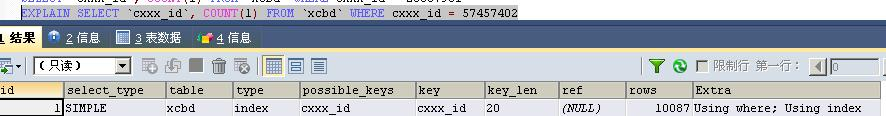
\includegraphics{0-2.jpg}


\subsection{使用汇总表}
\label{0/2:id3}
建立汇总表:

\begin{Verbatim}[commandchars=\\\{\}]
\PYG{k}{CREATE} \PYG{k}{TABLE} \PYG{l+s+ss}{{}`xcbd\PYGZus{}cxxx\PYGZus{}count{}`} \PYG{p}{(}
\PYG{l+s+ss}{{}`cxxx\PYGZus{}id{}`} \PYG{k+kt}{INT} \PYG{k}{PRIMARY} \PYG{k}{KEY}\PYG{p}{,}
\PYG{l+s+ss}{{}`count\PYGZus{}num{}`} \PYG{k+kt}{INT}
\PYG{p}{)}\PYG{p}{;}
\end{Verbatim}

定时插入数据进汇总表之前先清空汇总表:

\begin{Verbatim}[commandchars=\\\{\}]
\PYG{n}{TRUNCATE} \PYG{k}{TABLE} \PYG{n}{xcbd\PYGZus{}cxxx\PYGZus{}count}\PYG{p}{;}
\end{Verbatim}

定时插入数据进汇总表:

\begin{Verbatim}[commandchars=\\\{\}]
\PYG{k}{INSERT} \PYG{k}{INTO} \PYG{l+s+ss}{{}`xcbd\PYGZus{}cxxx\PYGZus{}count{}`} \PYG{p}{(}\PYG{l+s+ss}{{}`cxxx\PYGZus{}id{}`}\PYG{p}{,} \PYG{l+s+ss}{{}`count\PYGZus{}num{}`}\PYG{p}{)}
\PYG{k}{SELECT}
  \PYG{l+s+ss}{{}`cxxx\PYGZus{}id{}`}\PYG{p}{,}
  \PYG{n+nf}{COUNT}\PYG{p}{(}\PYG{l+m+mi}{1}\PYG{p}{)}
\PYG{k}{FROM}
  \PYG{l+s+ss}{{}`xcbd{}`}
\PYG{k}{GROUP} \PYG{k}{BY} \PYG{l+s+ss}{{}`cxxx\PYGZus{}id{}`} \PYG{p}{;}
\end{Verbatim}

查询汇总表数据:

\begin{Verbatim}[commandchars=\\\{\}]
\PYG{k}{SELECT}
  \PYG{n}{cxxx\PYGZus{}id}\PYG{p}{,}
  \PYG{n}{count\PYGZus{}num}
\PYG{k}{FROM}
  \PYG{n}{xcbd\PYGZus{}cxxx\PYGZus{}count}
\PYG{k}{WHERE} \PYG{n}{cxxx\PYGZus{}id} \PYG{o}{=} \PYG{l+m+mi}{23057901}
\end{Verbatim}

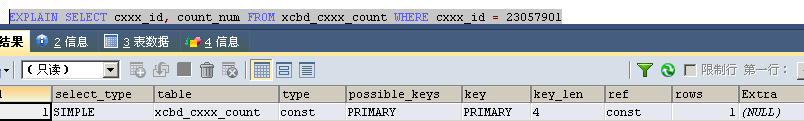
\includegraphics{0-3.png}


\section{禁止使用SELECT *,必须指定字段名称,包括insert table后边加字段列表}
\label{0/3:select-insert-table}\label{0/3::doc}
\begin{Verbatim}[commandchars=\\\{\}]
\PYG{k}{SELECT}
  \PYG{o}{*}
\PYG{k}{FROM}
  \PYG{n}{xcbd}
\PYG{k}{WHERE} \PYG{n}{cxxx\PYGZus{}id} \PYG{o}{=} \PYG{l+m+mi}{3}
\end{Verbatim}

正确做法:

\begin{Verbatim}[commandchars=\\\{\}]
\PYG{k}{SELECT}
  \PYG{n}{id}\PYG{p}{,}
  \PYG{n}{clxx\PYGZus{}id}\PYG{p}{,}
  \PYG{n}{cxxx\PYGZus{}id}\PYG{p}{,}
  \PYG{n}{qsd}\PYG{p}{,}
  \PYG{n}{zdd}
\PYG{k}{FROM}
  \PYG{n}{xcbd}
\PYG{k}{WHERE} \PYG{n}{cxxx\PYGZus{}id} \PYG{o}{=} \PYG{l+m+mi}{3}
\end{Verbatim}


\section{明细统计时,只统计编码,不要关联名称等冗余字段}
\label{0/4::doc}\label{0/4:id1}
\begin{Verbatim}[commandchars=\\\{\}]
\PYG{k}{SELECT}
  \PYG{n}{bd}\PYG{p}{.}\PYG{n}{clxx\PYGZus{}id}\PYG{p}{,}
  \PYG{n}{cl}\PYG{p}{.}\PYG{n}{cp}\PYG{p}{,}
  \PYG{n+nf}{COUNT}\PYG{p}{(}\PYG{n}{bd}\PYG{p}{.}\PYG{n}{clxx\PYGZus{}id}\PYG{p}{)}
\PYG{k}{FROM}
  \PYG{l+s+ss}{{}`xcbd{}`} \PYG{k}{AS} \PYG{n}{bd}
  \PYG{k}{INNER} \PYG{k}{JOIN} \PYG{n}{clxx} \PYG{k}{AS} \PYG{n}{cl}
    \PYG{k}{ON} \PYG{n}{bd}\PYG{p}{.}\PYG{n}{clxx\PYGZus{}id} \PYG{o}{=} \PYG{n}{cl}\PYG{p}{.}\PYG{n}{id}
\end{Verbatim}

或者

\begin{Verbatim}[commandchars=\\\{\}]
\PYG{k}{SELECT}
  \PYG{n}{clxx\PYGZus{}id}\PYG{p}{,}
  \PYG{n+nf}{COUNT}\PYG{p}{(}\PYG{l+m+mi}{1}\PYG{p}{)}\PYG{p}{,}
  \PYG{p}{(}\PYG{k}{SELECT}
    \PYG{n}{cp}
  \PYG{k}{FROM}
    \PYG{n}{clxx}
  \PYG{k}{WHERE} \PYG{n}{id} \PYG{o}{=} \PYG{n}{xcbd}\PYG{p}{.}\PYG{l+s+ss}{{}`clxx\PYGZus{}id{}`}\PYG{p}{)} \PYG{k}{AS} \PYG{n}{cp}
\PYG{k}{FROM}
  \PYG{l+s+ss}{{}`xcbd{}`}
\end{Verbatim}

正确做法

\begin{Verbatim}[commandchars=\\\{\}]
\PYG{k}{SELECT}
  \PYG{n}{clxx\PYGZus{}id}\PYG{p}{,}
  \PYG{n+nf}{COUNT}\PYG{p}{(}\PYG{l+m+mi}{1}\PYG{p}{)}
\PYG{k}{FROM}
  \PYG{l+s+ss}{{}`xcbd{}`}
\end{Verbatim}

取出结果后,根据实际情况再取cp。cp, id可以考虑运用缓存存储


\section{明细统计时,只统计编码,不要关联名称等冗余字段}
\label{0/5::doc}\label{0/5:id1}
\begin{Verbatim}[commandchars=\\\{\}]
\PYG{k}{SELECT}
  \PYG{n}{bd}\PYG{p}{.}\PYG{n}{clxx\PYGZus{}id}\PYG{p}{,}
  \PYG{n}{cl}\PYG{p}{.}\PYG{n}{cp}\PYG{p}{,}
  \PYG{n+nf}{COUNT}\PYG{p}{(}\PYG{n}{bd}\PYG{p}{.}\PYG{n}{clxx\PYGZus{}id}\PYG{p}{)}
\PYG{k}{FROM}
  \PYG{l+s+ss}{{}`xcbd{}`} \PYG{k}{AS} \PYG{n}{bd}
  \PYG{k}{INNER} \PYG{k}{JOIN} \PYG{n}{clxx} \PYG{k}{AS} \PYG{n}{cl}
    \PYG{k}{ON} \PYG{n}{bd}\PYG{p}{.}\PYG{n}{clxx\PYGZus{}id} \PYG{o}{=} \PYG{n}{cl}\PYG{p}{.}\PYG{n}{id}
\end{Verbatim}

或者

\begin{Verbatim}[commandchars=\\\{\}]
\PYG{k}{SELECT}
  \PYG{n}{clxx\PYGZus{}id}\PYG{p}{,}
  \PYG{n+nf}{COUNT}\PYG{p}{(}\PYG{l+m+mi}{1}\PYG{p}{)}\PYG{p}{,}
  \PYG{p}{(}\PYG{k}{SELECT}
    \PYG{n}{cp}
  \PYG{k}{FROM}
    \PYG{n}{clxx}
  \PYG{k}{WHERE} \PYG{n}{id} \PYG{o}{=} \PYG{n}{xcbd}\PYG{p}{.}\PYG{l+s+ss}{{}`clxx\PYGZus{}id{}`}\PYG{p}{)} \PYG{k}{AS} \PYG{n}{cp}
\PYG{k}{FROM}
  \PYG{l+s+ss}{{}`xcbd{}`}
\end{Verbatim}

正确做法

\begin{Verbatim}[commandchars=\\\{\}]
\PYG{k}{SELECT}
  \PYG{n}{clxx\PYGZus{}id}\PYG{p}{,}
  \PYG{n+nf}{COUNT}\PYG{p}{(}\PYG{l+m+mi}{1}\PYG{p}{)}
\PYG{k}{FROM}
  \PYG{l+s+ss}{{}`xcbd{}`}
\end{Verbatim}

取出结果后,根据实际情况再取cp。cp, id可以考虑运用缓存存储


\section{每个查询结果集使用的内存量不要超过256M,可以通过时间范围控制,如 RK BETWEEN A AND B,建议大表按可小时操作}
\label{0/6::doc}\label{0/6:m-rk-between-a-and-b}
\begin{Verbatim}[commandchars=\\\{\}]
\PYG{k}{SELECT}
  \PYG{n}{id}\PYG{p}{,}
  \PYG{n}{clxx\PYGZus{}id}\PYG{p}{,}
  \PYG{n}{cxxx\PYGZus{}id}\PYG{p}{,}
  \PYG{n}{qsd}\PYG{p}{,}
  \PYG{n}{zdd}
\PYG{k}{FROM}
  \PYG{n}{xcbd}
\PYG{k}{WHERE} \PYG{n}{del\PYGZus{}flag} \PYG{o}{=} \PYG{l+m+mi}{1}
\end{Verbatim}

改写为:

\begin{Verbatim}[commandchars=\\\{\}]
\PYG{k}{SELECT}
  \PYG{n}{id}\PYG{p}{,}
  \PYG{n}{clxx\PYGZus{}id}\PYG{p}{,}
  \PYG{n}{cxxx\PYGZus{}id}\PYG{p}{,}
  \PYG{n}{qsd}\PYG{p}{,}
  \PYG{n}{zdd}
\PYG{k}{FROM}
  \PYG{n}{xcbd}
\PYG{k}{WHERE} \PYG{n}{del\PYGZus{}flag} \PYG{o}{=} \PYG{l+m+mi}{1}
  \PYG{k}{AND} \PYG{n}{lrsj} \PYG{k}{BETWEEN} \PYG{p}{(}
    \PYG{l+s+s1}{\PYGZsq{}2012\PYGZhy{}01\PYGZhy{}01 00:00:00\PYGZsq{}}\PYG{p}{,}
    \PYG{l+s+s1}{\PYGZsq{}2012\PYGZhy{}01\PYGZhy{}02 00:00:00\PYGZsq{}}
  \PYG{p}{)}
\end{Verbatim}


\section{页面查询在10秒内要返回结果}
\label{0/7::doc}\label{0/7:id1}
页面查询在10秒内要返回结果,服务器超时限制默认是65秒(查看query cache是否足够大和命中率,show variables like `\%cache\%');


\section{联合查询时,每个表必须加别名以提高SQL解析效率}
\label{0/8::doc}\label{0/8:sql}
如 SELECT T1.BM FROM GS T1 LEFT JOIN GSJJ T2 ON T1.BM=T2.BM

\begin{Verbatim}[commandchars=\\\{\}]
\PYG{k}{SELECT}
  \PYG{n}{clxx\PYGZus{}id}\PYG{p}{,}
  \PYG{n}{cp}\PYG{p}{,}
  \PYG{n+nf}{COUNT}\PYG{p}{(}\PYG{n}{clxx\PYGZus{}id}\PYG{p}{)}
\PYG{k}{FROM}
  \PYG{l+s+ss}{{}`xcbd{}`} \PYG{n}{clxx}
\PYG{k}{WHERE} \PYG{n}{clxx\PYGZus{}id} \PYG{o}{=} \PYG{n}{id} \PYG{p}{;}
\end{Verbatim}

正确做法:

\begin{Verbatim}[commandchars=\\\{\}]
\PYG{k}{SELECT}
  \PYG{n}{bd}\PYG{p}{.}\PYG{n}{clxx\PYGZus{}id}\PYG{p}{,}
  \PYG{n}{cl}\PYG{p}{.}\PYG{n}{cp}\PYG{p}{,}
  \PYG{n+nf}{COUNT}\PYG{p}{(}\PYG{n}{bd}\PYG{p}{.}\PYG{n}{clxx\PYGZus{}id}\PYG{p}{)}
\PYG{k}{FROM}
  \PYG{l+s+ss}{{}`xcbd{}`} \PYG{k}{AS} \PYG{n}{bd} \PYG{p}{;}
  \PYG{k}{INNER} \PYG{k}{JOIN} \PYG{n}{clxx} \PYG{k}{AS} \PYG{n}{cl}
    \PYG{k}{ON} \PYG{n}{bd}\PYG{p}{.}\PYG{n}{clxx\PYGZus{}id} \PYG{o}{=} \PYG{n}{cl}\PYG{p}{.}\PYG{n}{id}
\end{Verbatim}


\section{语句中避免使用 GROUP BY, 可通过批量程序定期汇总}
\label{0/9:group-by}\label{0/9::doc}
\begin{Verbatim}[commandchars=\\\{\}]
\PYG{k}{SELECT}
  \PYG{n}{bd}\PYG{p}{.}\PYG{n}{clxx\PYGZus{}id}\PYG{p}{,}
  \PYG{n}{cl}\PYG{p}{.}\PYG{n}{cp}\PYG{p}{,}
  \PYG{n+nf}{COUNT}\PYG{p}{(}\PYG{n}{bd}\PYG{p}{.}\PYG{n}{clxx\PYGZus{}id}\PYG{p}{)}
\PYG{k}{FROM}
  \PYG{l+s+ss}{{}`xcbd{}`} \PYG{k}{AS} \PYG{n}{bd}
  \PYG{k}{INNER} \PYG{k}{JOIN} \PYG{n}{clxx} \PYG{k}{AS} \PYG{n}{cl}
    \PYG{k}{ON} \PYG{n}{bd}\PYG{p}{.}\PYG{n}{clxx\PYGZus{}id} \PYG{o}{=} \PYG{n}{cl}\PYG{p}{.}\PYG{n}{id}
\end{Verbatim}

或者

\begin{Verbatim}[commandchars=\\\{\}]
\PYG{k}{SELECT}
  \PYG{n}{clxx\PYGZus{}id}\PYG{p}{,}
  \PYG{n+nf}{COUNT}\PYG{p}{(}\PYG{l+m+mi}{1}\PYG{p}{)}\PYG{p}{,}
  \PYG{p}{(}\PYG{k}{SELECT}
    \PYG{n}{cp}
  \PYG{k}{FROM}
    \PYG{n}{clxx}
  \PYG{k}{WHERE} \PYG{n}{id} \PYG{o}{=} \PYG{n}{xcbd}\PYG{p}{.}\PYG{l+s+ss}{{}`clxx\PYGZus{}id{}`}\PYG{p}{)} \PYG{k}{AS} \PYG{n}{cp}
\PYG{k}{FROM}
  \PYG{l+s+ss}{{}`xcbd{}`}
\end{Verbatim}

正确做法

\begin{Verbatim}[commandchars=\\\{\}]
\PYG{k}{SELECT}
  \PYG{n}{clxx\PYGZus{}id}\PYG{p}{,}
  \PYG{n+nf}{COUNT}\PYG{p}{(}\PYG{l+m+mi}{1}\PYG{p}{)}
\PYG{k}{FROM}
  \PYG{l+s+ss}{{}`xcbd{}`}
\end{Verbatim}

取出结果后,根据实际情况再取cp。cp, id可以考虑运用缓存存储


\chapter{字段设计}
\label{1/0::doc}\label{1/0:id1}

\section{尽可能使用更小的数据类型,如 TINYINT、smallint,MEDIUMINT、INT、BIGINT (如int(11)的11代表客户端显示宽度,并不是取值范围,tinyint -2\textasciicircum{}8-2\textasciicircum{}8-1,smallint -2\textasciicircum{}15-2\textasciicircum{}15-1 int -2\textasciicircum{}31-2\textasciicircum{}31-1 bigint -2\textasciicircum{}63-2\textasciicircum{}63-1)}
\label{1/1:tinyintsmallint-mediumintintbigint-int-11-11-tinyint-2-8-2-8-1-smallint-2-15-2-15-1-int-2-31-2-31-1-bigint-2-63-2-63-1}\label{1/1::doc}
留空


\section{尽量少用 TEXT、BLOB 等专有类型   (用链接代替)}
\label{1/2:textblob}\label{1/2::doc}
留空


\section{字符型,数值型字段类型不能混合使用,依赖后期转换}
\label{1/3::doc}\label{1/3:id1}
留空


\section{相同字段不同表中的类型和长度要一致}
\label{1/4::doc}\label{1/4:id1}
留空


\section{字段名称不能使用关键字}
\label{1/5::doc}\label{1/5:id1}
留空


\section{不要指定字段级编码,建议全库统一}
\label{1/6::doc}\label{1/6:id1}
留空


\section{默认值要规范,例如日期不要使用 0000-00-00}
\label{1/7::doc}\label{1/7:id1}
留空


\section{不要用自增ID做主键}
\label{1/8::doc}\label{1/8:id}
留空


\section{不要使用外键}
\label{1/9::doc}\label{1/9:id1}
留空


\section{事务相关记录保留时间戳,建议只增不改;在必须对记录进行修改的时候,保留更改时间戳}
\label{1/10::doc}\label{1/10:id1}
留空


\chapter{索引使用}
\label{2/0::doc}\label{2/0:id1}

\section{一般情况下,一次查询只会用到一个索引 (特定情况出现merge index的情况,如下可能出现(a=1 or b=2)会合并a和b的索引,或者使用union all)}
\label{2/1:merge-index-a-1-or-b-2-ab-union-all}\label{2/1::doc}
explain mysql测试合并索引

建立索引:

\begin{Verbatim}[commandchars=\\\{\}]
\PYG{k}{CREATE} \PYG{k}{INDEX} \PYG{n}{emplyees\PYGZus{}firstname}
\PYG{k}{ON} \PYG{n+nf}{employees} \PYG{p}{(}\PYG{n}{first\PYGZus{}name}\PYG{p}{)}\PYG{p}{;}

\PYG{k}{CREATE} \PYG{k}{INDEX} \PYG{n}{emplyees\PYGZus{}lastname}
\PYG{k}{ON} \PYG{n+nf}{employees} \PYG{p}{(}\PYG{n}{last\PYGZus{}name}\PYG{p}{)}\PYG{p}{;}
\end{Verbatim}

a=1 or b=2 情况下:

\begin{Verbatim}[commandchars=\\\{\}]
\PYG{k}{EXPLAIN}
\PYG{k}{SELECT}
  \PYG{n}{emp\PYGZus{}no}\PYG{p}{,}
  \PYG{n}{birth\PYGZus{}date}\PYG{p}{,}
  \PYG{n}{first\PYGZus{}name}\PYG{p}{,}
  \PYG{n}{last\PYGZus{}name}\PYG{p}{,}
  \PYG{n}{gender} \PYG{n}{hire\PYGZus{}date}
\PYG{k}{FROM}
  \PYG{n}{employees}
\PYG{k}{WHERE} \PYG{n}{first\PYGZus{}name} \PYG{o}{=} \PYG{l+s+s1}{\PYGZsq{}Georgi\PYGZsq{}}
  \PYG{k}{OR} \PYG{n}{last\PYGZus{}name} \PYG{o}{=} \PYG{l+s+s1}{\PYGZsq{}Simmel\PYGZsq{}} \PYG{p}{;}
\end{Verbatim}

\begin{tabulary}{\linewidth}{|L|L|L|L|L|L|L|L|L|L|L|}
\hline
\textbf{
id
} & \textbf{
select\_type
} & \textbf{
table
} & \textbf{
type
} & \textbf{
possible\_keys
} & \textbf{
key
} & \textbf{
key\_len
} & \textbf{
ref
} & \textbf{
rows
} & \textbf{
filtered
} & \textbf{
Extra
}\\\hline

1
 & 
SIMPLE
 & 
employees
 & 
index\_merge
 & 
emplyees\_firstname,last\_name
 & 
emplyees\_firstname,last\_name
 & 
16,18
 &  & 
420
 & 
100.00
 & 
Using union(emplyees\_firstname,last\_name); Using where
\\\hline
\end{tabulary}


\begin{Verbatim}[commandchars=\\\{\}]
\PYG{k}{EXPLAIN} \PYG{n}{EXTENDED}
\PYG{k}{SELECT}
  \PYG{n}{emp\PYGZus{}no}\PYG{p}{,}
  \PYG{n}{birth\PYGZus{}date}\PYG{p}{,}
  \PYG{n}{first\PYGZus{}name}\PYG{p}{,}
  \PYG{n}{last\PYGZus{}name}\PYG{p}{,}
  \PYG{n}{gender} \PYG{n}{hire\PYGZus{}date}
\PYG{k}{FROM}
  \PYG{n}{employees}
\PYG{k}{WHERE} \PYG{n}{first\PYGZus{}name} \PYG{o}{=}  \PYG{l+s+s1}{\PYGZsq{}Georgi\PYGZsq{}}
\PYG{k}{UNION}
\PYG{k}{ALL}
\PYG{k}{SELECT}
  \PYG{n}{emp\PYGZus{}no}\PYG{p}{,}
  \PYG{n}{birth\PYGZus{}date}\PYG{p}{,}
  \PYG{n}{first\PYGZus{}name}\PYG{p}{,}
  \PYG{n}{last\PYGZus{}name}\PYG{p}{,}
  \PYG{n}{gender} \PYG{n}{hire\PYGZus{}date}
\PYG{k}{FROM}
  \PYG{n}{employees}
\PYG{k}{WHERE} \PYG{n}{last\PYGZus{}name} \PYG{o}{=} \PYG{l+s+s1}{\PYGZsq{}Simmel\PYGZsq{}} \PYG{p}{;}
\end{Verbatim}

\begin{tabulary}{\linewidth}{|L|L|L|L|L|L|L|L|L|L|L|}
\hline
\textbf{
id
} & \textbf{
select\_type
} & \textbf{
table
} & \textbf{
type
} & \textbf{
possible\_keys
} & \textbf{
key
} & \textbf{
key\_len
} & \textbf{
ref
} & \textbf{
rows
} & \textbf{
filtered
} & \textbf{
Extra
}\\\hline

1
 & 
PRIMARY
 & 
employees
 & 
ref
 & 
emplyees\_firstname
 & 
emplyees\_firstname
 & 
16
 & 
const
 & 
253
 & 
100.00
 & 
Using where
\\\hline

2
 & 
UNION
 & 
employees
 & 
ref
 & 
last\_name
 & 
last\_name
 & 
18
 & 
const
 & 
167
 & 
100.00
 & 
Using where
\\\hline
\end{tabulary}

\begin{itemize}
\item {} 
in与union:当条件参数为大量的时候,union all 明显慢于in

\end{itemize}

30W数据:
\begin{itemize}
\item {} 
无索引情况下:执行100条语句union耗时0.795秒,用in条件0.001秒

\item {} 
有索引情况下: 执行100条语句union耗时0.005秒,用in条件0.002秒

\end{itemize}

90W数据
\begin{itemize}
\item {} 
有索引情况下: 执行100条语句union耗时0.028秒,用in条件0.000秒

\end{itemize}

\begin{Verbatim}[commandchars=\\\{\}]
\PYG{k}{SELECT}
  \PYG{n}{emp\PYGZus{}no}\PYG{p}{,}
  \PYG{n}{birth\PYGZus{}date}\PYG{p}{,}
  \PYG{n}{first\PYGZus{}name}\PYG{p}{,}
  \PYG{n}{last\PYGZus{}name}\PYG{p}{,}
  \PYG{n}{gender} \PYG{n}{hire\PYGZus{}date}
\PYG{k}{FROM}
  \PYG{n}{employees}
\PYG{k}{WHERE} \PYG{n}{first\PYGZus{}name} \PYG{k}{IN} \PYG{p}{(}
    \PYG{l+s+s1}{\PYGZsq{}Georgi\PYGZsq{}}\PYG{p}{,}
    \PYG{l+s+s1}{\PYGZsq{}Bezalel\PYGZsq{}}\PYG{p}{,}
    \PYG{l+s+s1}{\PYGZsq{}Parto\PYGZsq{}}\PYG{p}{,}
    \PYG{l+s+s1}{\PYGZsq{}Chirstian\PYGZsq{}}\PYG{p}{,}
    \PYG{l+s+s1}{\PYGZsq{}Kyoichi\PYGZsq{}}\PYG{p}{,}
    \PYG{l+s+s1}{\PYGZsq{}Anneke\PYGZsq{}}\PYG{p}{,}
    \PYG{l+s+s1}{\PYGZsq{}Tzvetan\PYGZsq{}}\PYG{p}{,}
    \PYG{l+s+s1}{\PYGZsq{}Saniya\PYGZsq{}}\PYG{p}{,}
    \PYG{l+s+s1}{\PYGZsq{}Sumant\PYGZsq{}}\PYG{p}{,}
    \PYG{l+s+s1}{\PYGZsq{}Duangkaew\PYGZsq{}}\PYG{p}{,}
    \PYG{l+s+s1}{\PYGZsq{}Mary\PYGZsq{}}\PYG{p}{,}
    \PYG{l+s+s1}{\PYGZsq{}Patricio\PYGZsq{}}\PYG{p}{,}
    \PYG{l+s+s1}{\PYGZsq{}Eberhardt\PYGZsq{}}\PYG{p}{,}
    \PYG{l+s+s1}{\PYGZsq{}Berni\PYGZsq{}}\PYG{p}{,}
    \PYG{l+s+s1}{\PYGZsq{}Guoxiang\PYGZsq{}}\PYG{p}{,}
    \PYG{l+s+s1}{\PYGZsq{}Kazuhito\PYGZsq{}}\PYG{p}{,}
    \PYG{l+s+s1}{\PYGZsq{}Cristinel\PYGZsq{}}\PYG{p}{,}
    \PYG{l+s+s1}{\PYGZsq{}Kazuhide\PYGZsq{}}\PYG{p}{,}
    \PYG{l+s+s1}{\PYGZsq{}Lillian\PYGZsq{}}\PYG{p}{,}
    \PYG{l+s+s1}{\PYGZsq{}Mayuko\PYGZsq{}}\PYG{p}{,}
    \PYG{l+s+s1}{\PYGZsq{}Ramzi\PYGZsq{}}\PYG{p}{,}
    \PYG{l+s+s1}{\PYGZsq{}Shahaf\PYGZsq{}}\PYG{p}{,}
    \PYG{l+s+s1}{\PYGZsq{}Bojan\PYGZsq{}}\PYG{p}{,}
    \PYG{l+s+s1}{\PYGZsq{}Suzette\PYGZsq{}}\PYG{p}{,}
    \PYG{l+s+s1}{\PYGZsq{}Prasadram\PYGZsq{}}\PYG{p}{,}
    \PYG{l+s+s1}{\PYGZsq{}Yongqiao\PYGZsq{}}\PYG{p}{,}
    \PYG{l+s+s1}{\PYGZsq{}Divier\PYGZsq{}}\PYG{p}{,}
    \PYG{l+s+s1}{\PYGZsq{}Domenick\PYGZsq{}}\PYG{p}{,}
    \PYG{l+s+s1}{\PYGZsq{}Otmar\PYGZsq{}}\PYG{p}{,}
    \PYG{l+s+s1}{\PYGZsq{}Elvis\PYGZsq{}}\PYG{p}{,}
    \PYG{l+s+s1}{\PYGZsq{}Karsten\PYGZsq{}}\PYG{p}{,}
    \PYG{l+s+s1}{\PYGZsq{}Jeong\PYGZsq{}}\PYG{p}{,}
    \PYG{l+s+s1}{\PYGZsq{}Arif\PYGZsq{}}\PYG{p}{,}
    \PYG{l+s+s1}{\PYGZsq{}Bader\PYGZsq{}}\PYG{p}{,}
    \PYG{l+s+s1}{\PYGZsq{}Alain\PYGZsq{}}\PYG{p}{,}
    \PYG{l+s+s1}{\PYGZsq{}Adamantios\PYGZsq{}}\PYG{p}{,}
    \PYG{l+s+s1}{\PYGZsq{}Pradeep\PYGZsq{}}\PYG{p}{,}
    \PYG{l+s+s1}{\PYGZsq{}Huan\PYGZsq{}}\PYG{p}{,}
    \PYG{l+s+s1}{\PYGZsq{}Alejandro\PYGZsq{}}\PYG{p}{,}
    \PYG{l+s+s1}{\PYGZsq{}Weiyi\PYGZsq{}}\PYG{p}{,}
    \PYG{l+s+s1}{\PYGZsq{}Uri\PYGZsq{}}\PYG{p}{,}
    \PYG{l+s+s1}{\PYGZsq{}Magy\PYGZsq{}}\PYG{p}{,}
    \PYG{l+s+s1}{\PYGZsq{}Yishay\PYGZsq{}}\PYG{p}{,}
    \PYG{l+s+s1}{\PYGZsq{}Mingsen\PYGZsq{}}\PYG{p}{,}
    \PYG{l+s+s1}{\PYGZsq{}Moss\PYGZsq{}}\PYG{p}{,}
    \PYG{l+s+s1}{\PYGZsq{}Lucien\PYGZsq{}}\PYG{p}{,}
    \PYG{l+s+s1}{\PYGZsq{}Zvonko\PYGZsq{}}\PYG{p}{,}
    \PYG{l+s+s1}{\PYGZsq{}Florian\PYGZsq{}}\PYG{p}{,}
    \PYG{l+s+s1}{\PYGZsq{}Basil\PYGZsq{}}\PYG{p}{,}
    \PYG{l+s+s1}{\PYGZsq{}Yinghua\PYGZsq{}}\PYG{p}{,}
    \PYG{l+s+s1}{\PYGZsq{}Hidefumi\PYGZsq{}}\PYG{p}{,}
    \PYG{l+s+s1}{\PYGZsq{}Heping\PYGZsq{}}\PYG{p}{,}
    \PYG{l+s+s1}{\PYGZsq{}Sanjiv\PYGZsq{}}\PYG{p}{,}
    \PYG{l+s+s1}{\PYGZsq{}Mayumi\PYGZsq{}}\PYG{p}{,}
    \PYG{l+s+s1}{\PYGZsq{}Georgy\PYGZsq{}}\PYG{p}{,}
    \PYG{l+s+s1}{\PYGZsq{}Brendon\PYGZsq{}}\PYG{p}{,}
    \PYG{l+s+s1}{\PYGZsq{}Ebbe\PYGZsq{}}\PYG{p}{,}
    \PYG{l+s+s1}{\PYGZsq{}Berhard\PYGZsq{}}\PYG{p}{,}
    \PYG{l+s+s1}{\PYGZsq{}Breannda\PYGZsq{}}\PYG{p}{,}
    \PYG{l+s+s1}{\PYGZsq{}Tse\PYGZsq{}}\PYG{p}{,}
    \PYG{l+s+s1}{\PYGZsq{}Anoosh\PYGZsq{}}\PYG{p}{,}
    \PYG{l+s+s1}{\PYGZsq{}Gino\PYGZsq{}}\PYG{p}{,}
    \PYG{l+s+s1}{\PYGZsq{}Udi\PYGZsq{}}\PYG{p}{,}
    \PYG{l+s+s1}{\PYGZsq{}Satosi\PYGZsq{}}\PYG{p}{,}
    \PYG{l+s+s1}{\PYGZsq{}Kwee\PYGZsq{}}\PYG{p}{,}
    \PYG{l+s+s1}{\PYGZsq{}Claudi\PYGZsq{}}\PYG{p}{,}
    \PYG{l+s+s1}{\PYGZsq{}Charlene\PYGZsq{}}\PYG{p}{,}
    \PYG{l+s+s1}{\PYGZsq{}Margareta\PYGZsq{}}\PYG{p}{,}
    \PYG{l+s+s1}{\PYGZsq{}Reuven\PYGZsq{}}\PYG{p}{,}
    \PYG{l+s+s1}{\PYGZsq{}Hisao\PYGZsq{}}\PYG{p}{,}
    \PYG{l+s+s1}{\PYGZsq{}Hironoby\PYGZsq{}}\PYG{p}{,}
    \PYG{l+s+s1}{\PYGZsq{}Shir\PYGZsq{}}\PYG{p}{,}
    \PYG{l+s+s1}{\PYGZsq{}Mokhtar\PYGZsq{}}\PYG{p}{,}
    \PYG{l+s+s1}{\PYGZsq{}Gao\PYGZsq{}}\PYG{p}{,}
    \PYG{l+s+s1}{\PYGZsq{}Erez\PYGZsq{}}\PYG{p}{,}
    \PYG{l+s+s1}{\PYGZsq{}Mona\PYGZsq{}}\PYG{p}{,}
    \PYG{l+s+s1}{\PYGZsq{}Danel\PYGZsq{}}\PYG{p}{,}
    \PYG{l+s+s1}{\PYGZsq{}Kshitij\PYGZsq{}}\PYG{p}{,}
    \PYG{l+s+s1}{\PYGZsq{}Premal\PYGZsq{}}\PYG{p}{,}
    \PYG{l+s+s1}{\PYGZsq{}Zhongwei\PYGZsq{}}\PYG{p}{,}
    \PYG{l+s+s1}{\PYGZsq{}Parviz\PYGZsq{}}\PYG{p}{,}
    \PYG{l+s+s1}{\PYGZsq{}Vishv\PYGZsq{}}\PYG{p}{,}
    \PYG{l+s+s1}{\PYGZsq{}Tuval\PYGZsq{}}\PYG{p}{,}
    \PYG{l+s+s1}{\PYGZsq{}Kenroku\PYGZsq{}}\PYG{p}{,}
    \PYG{l+s+s1}{\PYGZsq{}Somnath\PYGZsq{}}\PYG{p}{,}
    \PYG{l+s+s1}{\PYGZsq{}Xinglin\PYGZsq{}}\PYG{p}{,}
    \PYG{l+s+s1}{\PYGZsq{}Jungsoon\PYGZsq{}}\PYG{p}{,}
    \PYG{l+s+s1}{\PYGZsq{}Sudharsan\PYGZsq{}}\PYG{p}{,}
    \PYG{l+s+s1}{\PYGZsq{}Kendra\PYGZsq{}}\PYG{p}{,}
    \PYG{l+s+s1}{\PYGZsq{}Amabile\PYGZsq{}}\PYG{p}{,}
    \PYG{l+s+s1}{\PYGZsq{}Valdiodio\PYGZsq{}}\PYG{p}{,}
    \PYG{l+s+s1}{\PYGZsq{}Sailaja\PYGZsq{}}\PYG{p}{,}
    \PYG{l+s+s1}{\PYGZsq{}Arumugam\PYGZsq{}}\PYG{p}{,}
    \PYG{l+s+s1}{\PYGZsq{}Hilari\PYGZsq{}}\PYG{p}{,}
    \PYG{l+s+s1}{\PYGZsq{}Jayson\PYGZsq{}}\PYG{p}{,}
    \PYG{l+s+s1}{\PYGZsq{}Remzi\PYGZsq{}}\PYG{p}{,}
    \PYG{l+s+s1}{\PYGZsq{}Sreekrishna\PYGZsq{}}\PYG{p}{,}
    \PYG{l+s+s1}{\PYGZsq{}Valter\PYGZsq{}}\PYG{p}{,}
    \PYG{l+s+s1}{\PYGZsq{}Hironobu\PYGZsq{}}\PYG{p}{,}
    \PYG{l+s+s1}{\PYGZsq{}Perla\PYGZsq{}}
  \PYG{p}{)}
\end{Verbatim}

无索引时扫描表100次

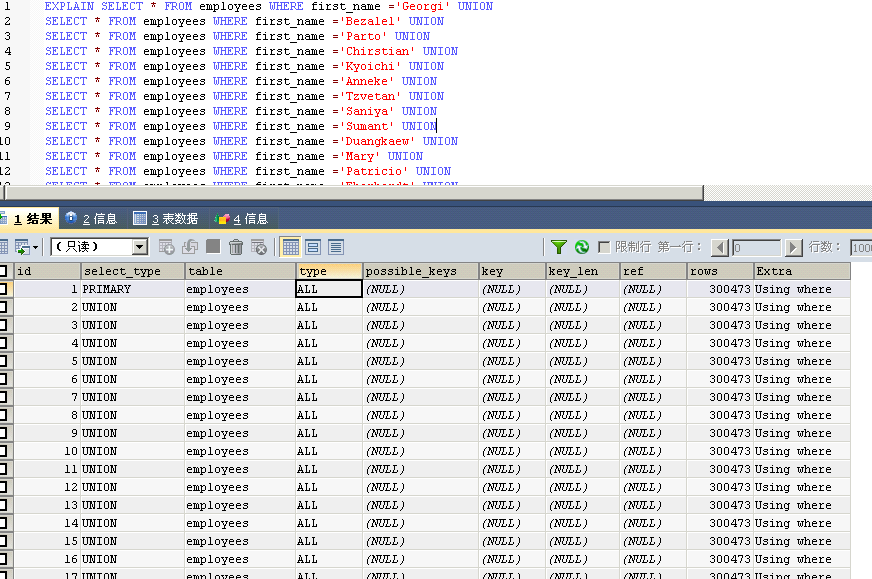
\includegraphics{3-1.png}


\section{每个表索引越少越好}
\label{2/2::doc}\label{2/2:id1}
每个表索引越少越好,建议1-3个,最多5个 (oltp 1-5,olap 5以上)


\section{每个查询必须用到索引}
\label{2/3::doc}\label{2/3:id1}
每个查询必须用到索引 (小表可能全表更好,视数据量决定)


\section{建立组合索引时,WHERE 条件中用到等于的字段放前边,用到范围的字段放后边}
\label{2/4:where}\label{2/4::doc}
建立组合索引时,WHERE 条件中用到等于的字段放前边,用到范围的字段放后边,如 DD=100000 AND SJ BETWEEN A AND B 例子(见以上)

explain mysql测试无左右条件左右说法


\section{删除重复字段的索引,减少dml IO}
\label{2/5:dml-io}\label{2/5::doc}
删除重复字段的索引,减少dml IO


\section{除了主键外,避免建立其他唯一性索引}
\label{2/6::doc}\label{2/6:id1}
除了主键外,避免建立其他唯一性索引

插入数据时增加额外开销


\section{索引中重复的记录数越少,效率越高,效率最高的是主键}
\label{2/7::doc}\label{2/7:id1}
索引中重复的记录数越少,效率越高,效率最高的是主键

如果同一记录超过50\%,全表扫描定期analyze table收集统计信息和直方图,如果可以加not null或者unique的最好加上


\section{索引字段最好不要存在 NULL}
\label{2/8:null}\label{2/8::doc}
索引字段最好不要存在 NULL,NULL可用 0 替代,建议把默认值设置为 0

也可以myisam\_stats\_method和innodb\_stats\_method取值nulls\_equal,在null远多于非null的情况下,建议表设计 default 0


\section{组合索引可以只使用第一个,或者前两个,或者前几个}
\label{2/9::doc}\label{2/9:id1}
组合索引可以只使用第一个,或者前两个,或者前几个,不能从第二个开始用,也不能跳着使用

索引使用从前缀开始,多字段索引到between或者\textless{},\textgreater{}等以后字段不会使用,排序最好在索引中实现

\begin{Verbatim}[commandchars=\\\{\}]
\PYG{k}{EXPLAIN}
\PYG{k}{SELECT}
  \PYG{n}{id}\PYG{p}{,}
  \PYG{n}{cxxx\PYGZus{}id}\PYG{p}{,}
  \PYG{n}{gs\PYGZus{}bm}\PYG{p}{,}
  \PYG{n}{gdddsj}\PYG{p}{,}
  \PYG{n}{gdlksj}
\PYG{k}{FROM}
  \PYG{n}{wdcx\PYGZus{}tjd}
\PYG{k}{WHERE} \PYG{n}{gs\PYGZus{}bm} \PYG{o}{=} \PYG{l+m+mi}{543001}
  \PYG{k}{AND} \PYG{n}{xh} \PYG{o}{=} \PYG{l+m+mi}{1}
\end{Verbatim}

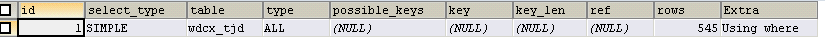
\includegraphics{3-2.png}

正确做法:

\begin{Verbatim}[commandchars=\\\{\}]
\PYG{k}{EXPLAIN}
\PYG{k}{SELECT}
  \PYG{n}{id}\PYG{p}{,}
  \PYG{n}{cxxx\PYGZus{}id}\PYG{p}{,}
  \PYG{n}{gs\PYGZus{}bm}\PYG{p}{,}
  \PYG{n}{gdddsj}\PYG{p}{,}
  \PYG{n}{gdlksj}
\PYG{k}{FROM}
  \PYG{n}{wdcx\PYGZus{}tjd}
\PYG{k}{WHERE} \PYG{n}{cxxx\PYGZus{}id} \PYG{o}{=} \PYG{l+m+mi}{9547}
  \PYG{k}{AND} \PYG{n}{xh} \PYG{o}{=} \PYG{l+m+mi}{1}
\end{Verbatim}

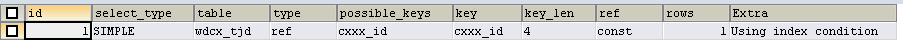
\includegraphics{3-3.png}

或者:

\begin{Verbatim}[commandchars=\\\{\}]
\PYG{k}{EXPLAIN}
\PYG{k}{SELECT}
  \PYG{n}{id}\PYG{p}{,}
  \PYG{n}{cxxx\PYGZus{}id}\PYG{p}{,}
  \PYG{n}{gs\PYGZus{}bm}\PYG{p}{,}
  \PYG{n}{gdddsj}\PYG{p}{,}
  \PYG{n}{gdlksj}
\PYG{k}{FROM}
  \PYG{n}{wdcx\PYGZus{}tjd}
\PYG{k}{WHERE} \PYG{n}{cxxx\PYGZus{}id} \PYG{o}{=} \PYG{l+m+mi}{9547}
  \PYG{k}{AND} \PYG{n}{gs\PYGZus{}bm} \PYG{o}{=} \PYG{l+m+mi}{543001}
  \PYG{k}{AND} \PYG{n}{xh} \PYG{o}{=} \PYG{l+m+mi}{1}
\end{Verbatim}

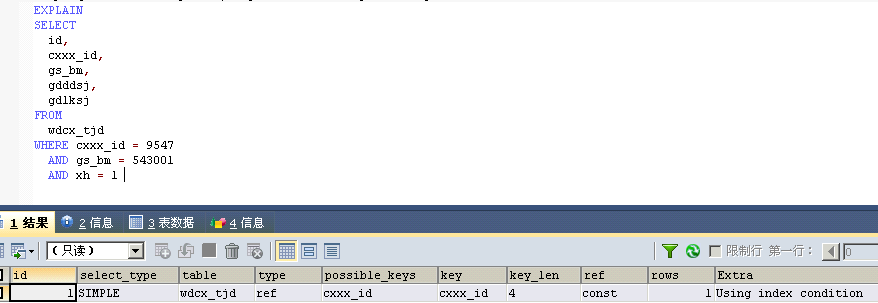
\includegraphics{3-4.png}


\chapter{查询条件}
\label{3/0::doc}\label{3/0:id1}

\section{SQL 语句的 WHERE 条件避免无效条件和无效括号}
\label{3/1::doc}\label{3/1:sql-where}
SQL 语句的 WHERE 条件避免无效条件和无效括号

如 SELECT BM FROM GS WHERE (1=1) 、 order by


\section{SQL语句中不要加用不到的排序}
\label{3/2::doc}\label{3/2:sql}
排序使用主键索引,比不排序多了读取索引的步骤

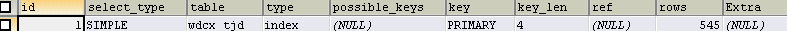
\includegraphics{4-1.png}

不使用索引:

\begin{Verbatim}[commandchars=\\\{\}]
\PYG{k}{EXPLAIN}
\PYG{k}{SELECT}
  \PYG{n}{id}\PYG{p}{,}
  \PYG{n}{cxxx\PYGZus{}id}\PYG{p}{,}
  \PYG{n}{gs\PYGZus{}bm}\PYG{p}{,}
  \PYG{n}{gdddsj}\PYG{p}{,}
  \PYG{n}{gdlksj}
\PYG{k}{FROM}
  \PYG{n}{wdcx\PYGZus{}tjd}
\end{Verbatim}

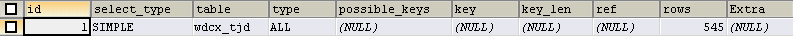
\includegraphics{4-2.png}


\section{WHERE 条件中 最好不要用 IN 和 LIKE}
\label{3/3:where-in-like}\label{3/3::doc}
WHERE 条件中 最好不要用 IN 和 LIKE

in的效率低于=。

无索引情况下,in效率要高于union。


\section{WHERE 条件中不要使用 NOW() 等进行判断}
\label{3/4::doc}\label{3/4:where-now}
WHERE 条件中不要使用 NOW() 等进行判断,影响执行计划


\section{索引要使用的字段不要使用函数或者进行运算}
\label{3/5::doc}\label{3/5:id1}
索引要使用的字段不要使用函数或者进行运算,如 field1 + 1 = field2、adddate(field1,…、CAST

\begin{Verbatim}[commandchars=\\\{\}]
\PYG{k}{EXPLAIN} \PYG{n}{EXTENDED}
\PYG{k}{SELECT}
  \PYG{p}{(}\PYG{n}{emp\PYGZus{}no} \PYG{o}{+} \PYG{l+m+mi}{100}\PYG{p}{)} \PYG{k}{AS} \PYG{n}{emp\PYGZus{}no100}\PYG{p}{,}
  \PYG{n}{birth\PYGZus{}date}\PYG{p}{,}
  \PYG{n+nf}{CONCAT}\PYG{p}{(}\PYG{n}{first\PYGZus{}name}
  \PYG{p}{,}\PYG{n}{last\PYGZus{}name}\PYG{p}{)} \PYG{k}{AS} \PYG{n}{fullname}\PYG{p}{,}
  \PYG{n}{gender} \PYG{n}{hire\PYGZus{}date}
\PYG{k}{FROM}
  \PYG{n}{employees}
\end{Verbatim}

运算方法,字符串连接,如无必要,在客户端中计算,连接。


\section{禁止字段格式转换}
\label{3/6::doc}\label{3/6:id1}
禁止字段格式转换,如 SELECT * FROM GS WHERE BM=200000,数值两边不要加引号

大多数字段使用函数不会使用索引,只有形如left(BM)=`200000'等可以使用)

查询条件和字段类型不一致,没有用到索引:

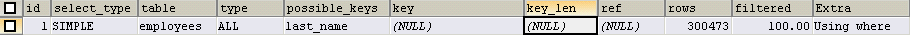
\includegraphics{4-3.png}

查询条件和字段类型不一致,用到索引:

\begin{Verbatim}[commandchars=\\\{\}]
\PYG{k}{EXPLAIN} \PYG{n}{EXTENDED}
\PYG{k}{SELECT}
  \PYG{n}{emp\PYGZus{}no}\PYG{p}{,}
  \PYG{n}{birth\PYGZus{}date}\PYG{p}{,}
  \PYG{n}{first\PYGZus{}name}\PYG{p}{,}
  \PYG{n}{last\PYGZus{}name}\PYG{p}{,}
  \PYG{n}{gender} \PYG{n}{hire\PYGZus{}date}
\PYG{k}{FROM}
  \PYG{n}{employees}
\PYG{k}{WHERE} \PYG{n}{last\PYGZus{}name}\PYG{o}{=}\PYG{l+s+s1}{\PYGZsq{}100001\PYGZsq{}}
\end{Verbatim}

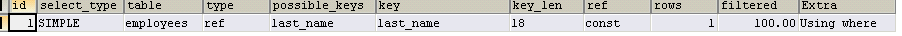
\includegraphics{4-4.png}


\chapter{存储过程}
\label{4/0::doc}\label{4/0:id1}

\section{存储过程中操作的记录数超过1000条时不能使用游标}
\label{4/1::doc}\label{4/1:id1}
存储过程中操作的记录数超过1000条时不能使用游标

禁止游标,用临时表代替

\begin{Verbatim}[commandchars=\\\{\}]
\PYG{k}{DELIMITER} \PYG{o}{/}\PYG{o}{/}
\PYG{k}{CREATE} \PYG{k}{PROCEDURE} \PYG{o}{{}`}\PYG{n}{curdemo}\PYG{o}{{}`}\PYG{p}{(}\PYG{p}{)}
\PYG{k}{BEGIN}
  \PYG{k}{DECLARE} \PYG{n}{done} \PYG{n+nb}{INT} \PYG{k}{DEFAULT} \PYG{l+m+mi}{0}\PYG{p}{;}
  \PYG{k}{DECLARE} \PYG{n}{a} \PYG{n+nb}{INT}\PYG{p}{;}
  \PYG{k}{DECLARE} \PYG{n}{b} \PYG{n+nb}{DATE}\PYG{p}{;}
  \PYG{k}{DECLARE} \PYG{n}{cur1} \PYG{k}{CURSOR} \PYG{k}{FOR} \PYG{k}{SELECT} \PYG{n}{emp\PYGZus{}no}\PYG{p}{,}\PYG{n}{hire\PYGZus{}date} \PYG{k}{FROM} \PYG{n}{employees} \PYG{k}{WHERE} \PYG{n}{first\PYGZus{}name}\PYG{o}{=}\PYG{l+s+s1}{\PYGZsq{}Georgi\PYGZsq{}}\PYG{p}{;}
  \PYG{k}{DECLARE} \PYG{k}{CONTINUE} \PYG{k}{HANDLER} \PYG{k}{FOR} \PYG{k}{SQLSTATE} \PYG{l+s+s1}{\PYGZsq{}02000\PYGZsq{}} \PYG{k}{SET} \PYG{n}{done} \PYG{o}{=} \PYG{l+m+mi}{1}\PYG{p}{;}
  \PYG{k}{OPEN} \PYG{n}{cur1}\PYG{p}{;}
  \PYG{n}{REPEAT}
    \PYG{k}{FETCH} \PYG{n}{cur1} \PYG{k}{INTO} \PYG{n}{a}\PYG{p}{,} \PYG{n}{b}\PYG{p}{;}
    \PYG{n}{IF} \PYG{k}{NOT} \PYG{n}{done} \PYG{k}{THEN}
       \PYG{n}{IF} \PYG{n}{hire\PYGZus{}date} \PYG{o}{\PYGZlt{}} \PYG{l+s+s1}{\PYGZsq{}1989\PYGZhy{}10\PYGZhy{}01\PYGZsq{}} \PYG{k}{THEN}
          \PYG{k}{INSERT} \PYG{k}{INTO} \PYG{n}{tmp1} \PYG{p}{(}\PYG{n}{emp\PYGZus{}no}\PYG{p}{)} \PYG{k}{VALUES} \PYG{p}{(}\PYG{n}{vemp\PYGZus{}no}\PYG{p}{)}\PYG{p}{;}
       \PYG{k}{ELSE}
          \PYG{k}{INSERT} \PYG{k}{INTO} \PYG{n}{tmp2} \PYG{p}{(}\PYG{n}{emp\PYGZus{}no}\PYG{p}{)} \PYG{k}{VALUES} \PYG{p}{(}\PYG{n}{vemp\PYGZus{}no}\PYG{p}{)}
       \PYG{k}{END} \PYG{n}{IF}\PYG{p}{;}
    \PYG{k}{END} \PYG{n}{IF}\PYG{p}{;}
  \PYG{k}{UNTIL} \PYG{n}{done} \PYG{k}{END} \PYG{n}{REPEAT}\PYG{p}{;}
  \PYG{k}{CLOSE} \PYG{n}{cur1}\PYG{p}{;}
\PYG{k}{END} \PYG{o}{/}\PYG{o}{/}
\PYG{k}{DELIMITER} \PYG{p}{;}
\end{Verbatim}

建立临时表:

\begin{Verbatim}[commandchars=\\\{\}]
\PYG{n}{DELIMITER} \PYG{o}{/}\PYG{o}{/}
\PYG{k}{CREATE} \PYG{k}{PROCEDURE} \PYG{l+s+ss}{{}`curdemo{}`}\PYG{p}{(}\PYG{p}{)}
\PYG{n}{BEGIN}
\PYG{k}{INSERT} \PYG{k}{INTO} \PYG{n+nf}{tmp\PYGZus{}table}  \PYG{p}{(}\PYG{n}{emp\PYGZus{}no}\PYG{p}{,} \PYG{n}{hire\PYGZus{}date}\PYG{p}{)} \PYG{k}{SELECT} \PYG{n}{emp\PYGZus{}no}\PYG{p}{,}\PYG{n}{hire\PYGZus{}date} \PYG{k}{FROM} \PYG{n}{employees} \PYG{k}{WHERE} \PYG{n}{first\PYGZus{}name}\PYG{o}{=}\PYG{l+s+s1}{\PYGZsq{}Georgi\PYGZsq{}}\PYG{p}{;}

\PYG{k}{INSERT} \PYG{k}{INTO} \PYG{n+nf}{tmp1} \PYG{p}{(}\PYG{n}{emp\PYGZus{}no}\PYG{p}{)} \PYG{k}{SELECT} \PYG{n}{emp\PYGZus{}no} \PYG{k}{FROM} \PYG{n}{tmp\PYGZus{}table} \PYG{k}{WHERE} \PYG{n}{hire\PYGZus{}date} \PYG{o}{\PYGZlt{}} \PYG{l+s+s1}{\PYGZsq{}1989\PYGZhy{}10\PYGZhy{}01\PYGZsq{}} \PYG{p}{;}
\PYG{k}{INSERT} \PYG{k}{INTO} \PYG{n+nf}{tmp2} \PYG{p}{(}\PYG{n}{emp\PYGZus{}no}\PYG{p}{)} \PYG{k}{SELECT} \PYG{n}{emp\PYGZus{}no} \PYG{k}{FROM} \PYG{n}{tmp\PYGZus{}table} \PYG{k}{WHERE} \PYG{n}{hire\PYGZus{}date} \PYG{o}{\PYGZgt{}}\PYG{o}{=}\PYG{l+s+s1}{\PYGZsq{}1989\PYGZhy{}10\PYGZhy{}01\PYGZsq{}} \PYG{p}{;}
\PYG{n}{END} \PYG{o}{/}\PYG{o}{/}
\PYG{n}{DELIMITER} \PYG{p}{;}
\end{Verbatim}


\section{在存储过程的关键步骤开始和结束都要记录信息到日志表,用于监控和调试}
\label{4/2::doc}\label{4/2:id1}
在存储过程的关键步骤开始和结束都要记录信息到日志表,用于监控和调试

建立日志表:

\begin{Verbatim}[commandchars=\\\{\}]
\PYG{k}{CREATE} \PYG{k}{TABLE} \PYG{l+s+ss}{{}`mylogs{}`} \PYG{p}{(}
  \PYG{l+s+ss}{{}`produce\PYGZus{}name{}`} \PYG{k+kt}{CHAR}\PYG{p}{(}\PYG{l+m+mi}{20}\PYG{p}{)} \PYG{k}{DEFAULT} \PYG{n+no}{NULL}\PYG{p}{,}
  \PYG{l+s+ss}{{}`dt{}`} \PYG{k+kt}{DATETIME} \PYG{k}{DEFAULT} \PYG{n+no}{NULL}\PYG{p}{,}
  \PYG{l+s+ss}{{}`step{}`} \PYG{k+kt}{SMALLINT}\PYG{p}{(}\PYG{l+m+mi}{6}\PYG{p}{)} \PYG{k}{DEFAULT} \PYG{n+no}{NULL}\PYG{p}{,}
  \PYG{l+s+ss}{{}`msg{}`} \PYG{k+kt}{VARCHAR}\PYG{p}{(}\PYG{l+m+mi}{100}\PYG{p}{)} \PYG{k}{DEFAULT} \PYG{n+no}{NULL}\PYG{p}{,}
  \PYG{k}{KEY} \PYG{l+s+ss}{{}`produce\PYGZus{}name{}`} \PYG{p}{(}\PYG{l+s+ss}{{}`produce\PYGZus{}name{}`}\PYG{p}{,}\PYG{l+s+ss}{{}`dt{}`}\PYG{p}{)}
\PYG{p}{)}

\PYG{n}{DELIMITER} \PYG{o}{/}\PYG{o}{/}
\PYG{k}{CREATE} \PYG{k}{PROCEDURE} \PYG{l+s+ss}{{}`curdemo{}`} \PYG{p}{(}\PYG{p}{)}
\PYG{n}{BEGIN}
  \PYG{k}{INSERT} \PYG{k}{INTO} \PYG{n+nf}{mylogs} \PYG{p}{(}\PYG{l+s+ss}{{}`produce\PYGZus{}name{}`}\PYG{p}{,} \PYG{l+s+ss}{{}`dt{}`}\PYG{p}{,} \PYG{l+s+ss}{{}`step{}`}\PYG{p}{,} \PYG{l+s+ss}{{}`msg{}`}\PYG{p}{)}
  \PYG{k}{VALUES}
    \PYG{p}{(}
      \PYG{n}{procedure\PYGZus{}name}\PYG{p}{,}
      \PYG{n+nf}{NOW}\PYG{p}{(}\PYG{p}{)}\PYG{p}{,}
      \PYG{l+m+mi}{0}\PYG{p}{,}
      \PYG{l+s+s1}{\PYGZsq{}程序开始\PYGZsq{}}
    \PYG{p}{)} \PYG{p}{;}
  \PYG{k}{DECLARE} \PYG{n}{done} \PYG{k+kt}{INT} \PYG{k}{DEFAULT} \PYG{l+m+mi}{0} \PYG{p}{;}
  \PYG{k}{DECLARE} \PYG{n}{procedure\PYGZus{}name} \PYG{k+kt}{CHAR}\PYG{p}{(}\PYG{l+m+mi}{20}\PYG{p}{)} \PYG{p}{;}
  \PYG{k+kt}{SET} \PYG{n}{procedure\PYGZus{}name} \PYG{o}{=} \PYG{l+s+s1}{\PYGZsq{}curdemo\PYGZsq{}} \PYG{p}{;}
  \PYG{k}{DECLARE} \PYG{n}{a} \PYG{k+kt}{INT} \PYG{p}{;}
  \PYG{k}{DECLARE} \PYG{n}{b} \PYG{k+kt}{DATE} \PYG{p}{;}
  \PYG{k}{DECLARE} \PYG{n}{cur1} \PYG{k}{CURSOR} \PYG{k}{FOR}
  \PYG{k}{SELECT}
    \PYG{n}{emp\PYGZus{}no}\PYG{p}{,}
    \PYG{n}{hire\PYGZus{}date}
  \PYG{k}{FROM}
    \PYG{n}{employees}
  \PYG{k}{WHERE} \PYG{n}{first\PYGZus{}name} \PYG{o}{=} \PYG{l+s+s1}{\PYGZsq{}Georgi\PYGZsq{}} \PYG{p}{;}
  \PYG{k}{DECLARE} \PYG{k}{CONTINUE} \PYG{n}{HANDLER} \PYG{k}{FOR} \PYG{k}{SQLSTATE} \PYG{l+s+s1}{\PYGZsq{}02000\PYGZsq{}} \PYG{k+kt}{SET} \PYG{n}{done} \PYG{o}{=} \PYG{l+m+mi}{1} \PYG{p}{;}
  \PYG{k}{INSERT} \PYG{k}{INTO} \PYG{n+nf}{mylogs} \PYG{p}{(}\PYG{l+s+ss}{{}`produce\PYGZus{}name{}`}\PYG{p}{,} \PYG{l+s+ss}{{}`dt{}`}\PYG{p}{,} \PYG{l+s+ss}{{}`step{}`}\PYG{p}{,} \PYG{l+s+ss}{{}`msg{}`}\PYG{p}{)}
  \PYG{k}{VALUES}
    \PYG{p}{(}
      \PYG{n}{procedure\PYGZus{}name}\PYG{p}{,}
      \PYG{n+nf}{NOW}\PYG{p}{(}\PYG{p}{)}\PYG{p}{,}
      \PYG{l+m+mi}{1}\PYG{p}{,}
      \PYG{l+s+s1}{\PYGZsq{}开始打开游标\PYGZsq{}}
    \PYG{p}{)} \PYG{p}{;}
  \PYG{n}{OPEN} \PYG{n}{cur1} \PYG{p}{;}
  \PYG{k}{INSERT} \PYG{k}{INTO} \PYG{n+nf}{mylogs} \PYG{p}{(}\PYG{l+s+ss}{{}`produce\PYGZus{}name{}`}\PYG{p}{,} \PYG{l+s+ss}{{}`dt{}`}\PYG{p}{,} \PYG{l+s+ss}{{}`step{}`}\PYG{p}{,} \PYG{l+s+ss}{{}`msg{}`}\PYG{p}{)}
  \PYG{k}{VALUES}
    \PYG{p}{(}
      \PYG{n}{procedure\PYGZus{}name}\PYG{p}{,}
      \PYG{n+nf}{NOW}\PYG{p}{(}\PYG{p}{)}\PYG{p}{,}
      \PYG{l+m+mi}{2}\PYG{p}{,}
      \PYG{l+s+s1}{\PYGZsq{}结束打开游标\PYGZsq{}}
    \PYG{p}{)} \PYG{p}{;}
  \PYG{k}{INSERT} \PYG{k}{INTO} \PYG{n+nf}{mylogs} \PYG{p}{(}\PYG{l+s+ss}{{}`produce\PYGZus{}name{}`}\PYG{p}{,} \PYG{l+s+ss}{{}`dt{}`}\PYG{p}{,} \PYG{l+s+ss}{{}`step{}`}\PYG{p}{,} \PYG{l+s+ss}{{}`msg{}`}\PYG{p}{)}
  \PYG{k}{VALUES}
    \PYG{p}{(}
      \PYG{n}{procedure\PYGZus{}name}\PYG{p}{,}
      \PYG{n+nf}{NOW}\PYG{p}{(}\PYG{p}{)}\PYG{p}{,}
      \PYG{l+m+mi}{3}\PYG{p}{,}
      \PYG{l+s+s1}{\PYGZsq{}开始处理数据\PYGZsq{}}
    \PYG{p}{)} \PYG{p}{;}
  \PYG{k}{REPEAT}
    \PYG{k}{FETCH} \PYG{n}{cur1} \PYG{k}{INTO} \PYG{n}{a}\PYG{p}{,}
    \PYG{n}{b} \PYG{p}{;}
    \PYG{k}{IF} \PYG{k}{NOT} \PYG{n}{done}
    \PYG{k}{THEN} \PYG{k}{IF} \PYG{n}{hire\PYGZus{}date} \PYG{o}{\PYGZlt{}} \PYG{l+s+s1}{\PYGZsq{}1989\PYGZhy{}10\PYGZhy{}01\PYGZsq{}}
    \PYG{k}{THEN}
    \PYG{k}{INSERT} \PYG{k}{INTO} \PYG{n+nf}{tmp1} \PYG{p}{(}\PYG{n}{emp\PYGZus{}no}\PYG{p}{)}
    \PYG{k}{VALUES}
      \PYG{p}{(}\PYG{n}{vemp\PYGZus{}no}\PYG{p}{)} \PYG{p}{;}
    \PYG{k}{ELSE}
    \PYG{k}{INSERT} \PYG{k}{INTO} \PYG{n+nf}{tmp2} \PYG{p}{(}\PYG{n}{emp\PYGZus{}no}\PYG{p}{)}
    \PYG{k}{VALUES}
      \PYG{p}{(}\PYG{n}{vemp\PYGZus{}no}\PYG{p}{)} \PYG{n}{END} \PYG{k}{IF} \PYG{p}{;}
    \PYG{n}{END} \PYG{k}{IF} \PYG{p}{;}
    \PYG{n}{UNTIL} \PYG{n}{done}
  \PYG{n}{END} \PYG{k}{REPEAT} \PYG{p}{;}
  \PYG{k}{INSERT} \PYG{k}{INTO} \PYG{n+nf}{mylogs} \PYG{p}{(}\PYG{l+s+ss}{{}`produce\PYGZus{}name{}`}\PYG{p}{,} \PYG{l+s+ss}{{}`dt{}`}\PYG{p}{,} \PYG{l+s+ss}{{}`step{}`}\PYG{p}{,} \PYG{l+s+ss}{{}`msg{}`}\PYG{p}{)}
  \PYG{k}{VALUES}
    \PYG{p}{(}
      \PYG{n}{procedure\PYGZus{}name}\PYG{p}{,}
      \PYG{n+nf}{NOW}\PYG{p}{(}\PYG{p}{)}\PYG{p}{,}
      \PYG{l+m+mi}{4}\PYG{p}{,}
      \PYG{l+s+s1}{\PYGZsq{}结束处理数据\PYGZsq{}}
    \PYG{p}{)} \PYG{p}{;}
  \PYG{k}{INSERT} \PYG{k}{INTO} \PYG{n+nf}{mylogs} \PYG{p}{(}\PYG{l+s+ss}{{}`produce\PYGZus{}name{}`}\PYG{p}{,} \PYG{l+s+ss}{{}`dt{}`}\PYG{p}{,} \PYG{l+s+ss}{{}`step{}`}\PYG{p}{,} \PYG{l+s+ss}{{}`msg{}`}\PYG{p}{)}
  \PYG{k}{VALUES}
    \PYG{p}{(}
      \PYG{n}{procedure\PYGZus{}name}\PYG{p}{,}
      \PYG{n+nf}{NOW}\PYG{p}{(}\PYG{p}{)}\PYG{p}{,}
      \PYG{l+m+mi}{5}\PYG{p}{,}
      \PYG{l+s+s1}{\PYGZsq{}关闭游标\PYGZsq{}}
    \PYG{p}{)} \PYG{p}{;}
  \PYG{n}{CLOSE} \PYG{n}{cur1} \PYG{p}{;}
  \PYG{k}{INSERT} \PYG{k}{INTO} \PYG{n+nf}{mylogs} \PYG{p}{(}\PYG{l+s+ss}{{}`produce\PYGZus{}name{}`}\PYG{p}{,} \PYG{l+s+ss}{{}`dt{}`}\PYG{p}{,} \PYG{l+s+ss}{{}`step{}`}\PYG{p}{,} \PYG{l+s+ss}{{}`msg{}`}\PYG{p}{)}
  \PYG{k}{VALUES}
    \PYG{p}{(}
      \PYG{n}{procedure\PYGZus{}name}\PYG{p}{,}
      \PYG{n+nf}{NOW}\PYG{p}{(}\PYG{p}{)}\PYG{p}{,}
      \PYG{l+m+mi}{6}\PYG{p}{,}
      \PYG{l+s+s1}{\PYGZsq{}程序结束\PYGZsq{}}
    \PYG{p}{)} \PYG{p}{;}
\PYG{n}{END} \PYG{o}{/}\PYG{o}{/}

\PYG{n}{DELIMITER} \PYG{p}{;}
\end{Verbatim}

\emph{INSERT INTO mylogs 可以写一个存储过程,以增加可读性。}

\begin{Verbatim}[commandchars=\\\{\}]
\PYG{n}{DELIMITER} \PYG{o}{/}\PYG{o}{/}
\PYG{k}{CREATE} \PYG{k}{PROCEDURE} \PYG{l+s+ss}{{}`writelogs{}`} \PYG{p}{(}
  \PYG{k}{IN} \PYG{n}{produce\PYGZus{}name} \PYG{k+kt}{CHAR}\PYG{p}{(}\PYG{l+m+mi}{20}\PYG{p}{)}\PYG{p}{,}
  \PYG{k}{IN} \PYG{n}{step} \PYG{k+kt}{SMALLINT}\PYG{p}{,}
  \PYG{k}{IN} \PYG{n}{msg} \PYG{k+kt}{CHAR}\PYG{p}{(}\PYG{l+m+mi}{100}\PYG{p}{)}
\PYG{p}{)}
\PYG{n}{BEGIN}
  \PYG{k}{INSERT} \PYG{k}{INTO} \PYG{n+nf}{mylogs} \PYG{p}{(}\PYG{l+s+ss}{{}`produce\PYGZus{}name{}`}\PYG{p}{,} \PYG{l+s+ss}{{}`dt{}`}\PYG{p}{,} \PYG{l+s+ss}{{}`step{}`}\PYG{p}{,} \PYG{l+s+ss}{{}`msg{}`}\PYG{p}{)}
  \PYG{k}{VALUES}
    \PYG{p}{(}\PYG{n}{produce\PYGZus{}name}\PYG{p}{,} \PYG{n+nf}{NOW}\PYG{p}{(}\PYG{p}{)}\PYG{p}{,} \PYG{n}{step}\PYG{p}{,} \PYG{n}{msg}\PYG{p}{)} \PYG{p}{;}
\PYG{n}{END} \PYG{o}{/}\PYG{o}{/}
\PYG{n}{DELIMITER} \PYG{p}{;}
\end{Verbatim}

程序改写后:

\begin{Verbatim}[commandchars=\\\{\}]
\PYG{n}{DELIMITER} \PYG{o}{/}\PYG{o}{/}
\PYG{k}{CREATE} \PYG{k}{PROCEDURE} \PYG{l+s+ss}{{}`curdemo{}`} \PYG{p}{(}\PYG{p}{)}
\PYG{n}{BEGIN}
  \PYG{k}{DECLARE} \PYG{n}{procedure\PYGZus{}name} \PYG{k+kt}{CHAR}\PYG{p}{(}\PYG{l+m+mi}{20}\PYG{p}{)} \PYG{k}{DEFAULT} \PYG{l+s+s1}{\PYGZsq{}curdemo\PYGZsq{}} \PYG{p}{;}
  \PYG{k}{DECLARE} \PYG{n}{done} \PYG{k+kt}{INT} \PYG{k}{DEFAULT} \PYG{l+m+mi}{0} \PYG{p}{;}
  \PYG{k}{DECLARE} \PYG{n}{a} \PYG{k+kt}{INT} \PYG{p}{;}
  \PYG{k}{DECLARE} \PYG{n}{b} \PYG{k+kt}{DATE} \PYG{p}{;}
  \PYG{k}{DECLARE} \PYG{n}{cur1} \PYG{k}{CURSOR} \PYG{k}{FOR}
  \PYG{k}{SELECT}
    \PYG{n}{emp\PYGZus{}no}\PYG{p}{,}
    \PYG{n}{hire\PYGZus{}date}
  \PYG{k}{FROM}
    \PYG{n}{employees}
  \PYG{k}{WHERE} \PYG{n}{first\PYGZus{}name} \PYG{o}{=} \PYG{l+s+s1}{\PYGZsq{}Georgi\PYGZsq{}} \PYG{p}{;}
  \PYG{k}{DECLARE} \PYG{k}{CONTINUE} \PYG{n}{HANDLER} \PYG{k}{FOR} \PYG{k}{SQLSTATE} \PYG{l+s+s1}{\PYGZsq{}02000\PYGZsq{}} \PYG{k+kt}{SET} \PYG{n}{done} \PYG{o}{=} \PYG{l+m+mi}{1} \PYG{p}{;}
  \PYG{k}{CALL} \PYG{n+nf}{writelogs} \PYG{p}{(}\PYG{n}{procedure\PYGZus{}name}\PYG{p}{,} \PYG{l+m+mi}{0}\PYG{p}{,} \PYG{l+s+s1}{\PYGZsq{}程序开始\PYGZsq{}}\PYG{p}{)} \PYG{p}{;}
  \PYG{k}{CALL} \PYG{n+nf}{writelogs} \PYG{p}{(}
    \PYG{n}{procedure\PYGZus{}name}\PYG{p}{,}
    \PYG{l+m+mi}{1}\PYG{p}{,}
    \PYG{l+s+s1}{\PYGZsq{}开始打开游标\PYGZsq{}}
  \PYG{p}{)} \PYG{p}{;}
  \PYG{n}{OPEN} \PYG{n}{cur1} \PYG{p}{;}
  \PYG{k}{CALL} \PYG{n+nf}{writelogs} \PYG{p}{(}
    \PYG{n}{procedure\PYGZus{}name}\PYG{p}{,}
    \PYG{l+m+mi}{2}\PYG{p}{,}
    \PYG{l+s+s1}{\PYGZsq{}结束打开游标\PYGZsq{}}
  \PYG{p}{)} \PYG{p}{;}
  \PYG{k}{CALL} \PYG{n+nf}{writelogs} \PYG{p}{(}
    \PYG{n}{procedure\PYGZus{}name}\PYG{p}{,}
    \PYG{l+m+mi}{3}\PYG{p}{,}
    \PYG{l+s+s1}{\PYGZsq{}开始处理数据\PYGZsq{}}
  \PYG{p}{)} \PYG{p}{;}
  \PYG{k}{REPEAT}
    \PYG{k}{FETCH} \PYG{n}{cur1} \PYG{k}{INTO} \PYG{n}{a}\PYG{p}{,}
    \PYG{n}{b} \PYG{p}{;}
    \PYG{k}{IF} \PYG{k}{NOT} \PYG{n}{done}
    \PYG{k}{THEN} \PYG{k}{IF} \PYG{n}{hire\PYGZus{}date} \PYG{o}{\PYGZlt{}} \PYG{l+s+s1}{\PYGZsq{}1989\PYGZhy{}10\PYGZhy{}01\PYGZsq{}}
    \PYG{k}{THEN}
    \PYG{k}{INSERT} \PYG{k}{INTO} \PYG{n+nf}{tmp1} \PYG{p}{(}\PYG{n}{emp\PYGZus{}no}\PYG{p}{)}
    \PYG{k}{VALUES}
      \PYG{p}{(}\PYG{n}{vemp\PYGZus{}no}\PYG{p}{)} \PYG{p}{;}
    \PYG{k}{ELSE}
    \PYG{k}{INSERT} \PYG{k}{INTO} \PYG{n+nf}{tmp2} \PYG{p}{(}\PYG{n}{emp\PYGZus{}no}\PYG{p}{)}
    \PYG{k}{VALUES}
      \PYG{p}{(}\PYG{n}{vemp\PYGZus{}no}\PYG{p}{)} \PYG{p}{;}
    \PYG{n}{END} \PYG{k}{IF} \PYG{p}{;}
    \PYG{n}{END} \PYG{k}{IF} \PYG{p}{;}
    \PYG{n}{UNTIL} \PYG{n}{done}
  \PYG{n}{END} \PYG{k}{REPEAT} \PYG{p}{;}
  \PYG{k}{CALL} \PYG{n+nf}{writelogs} \PYG{p}{(}
    \PYG{n}{procedure\PYGZus{}name}\PYG{p}{,}
    \PYG{l+m+mi}{4}\PYG{p}{,}
    \PYG{l+s+s1}{\PYGZsq{}结束处理数据\PYGZsq{}}
  \PYG{p}{)} \PYG{p}{;}
  \PYG{k}{CALL} \PYG{n+nf}{writelogs} \PYG{p}{(}\PYG{n}{procedure\PYGZus{}name}\PYG{p}{,} \PYG{l+m+mi}{5}\PYG{p}{,} \PYG{l+s+s1}{\PYGZsq{}关闭游标\PYGZsq{}}\PYG{p}{)} \PYG{p}{;}
  \PYG{n}{CLOSE} \PYG{n}{cur1} \PYG{p}{;}
  \PYG{k}{CALL} \PYG{n+nf}{writelogs} \PYG{p}{(}\PYG{n}{procedure\PYGZus{}name}\PYG{p}{,} \PYG{l+m+mi}{6}\PYG{p}{,} \PYG{l+s+s1}{\PYGZsq{}程序结束\PYGZsq{}}\PYG{p}{)} \PYG{p}{;}
\PYG{n}{END} \PYG{o}{/}\PYG{o}{/}

\PYG{n}{DELIMITER} \PYG{p}{;}
\end{Verbatim}


\section{字符变量使用单引号,不要使用双引号}
\label{4/3::doc}\label{4/3:id1}
字符变量使用单引号,不要使用双引号,【''2012-09-23 00:00:00''】 可改为 【`2012-09-23 00:00:00'】

\begin{Verbatim}[commandchars=\\\{\}]
\PYG{k}{SELECT} \PYG{n}{emp\PYGZus{}no}\PYG{p}{,} \PYG{n}{first\PYGZus{}name}\PYG{p}{,} \PYG{n}{last\PYGZus{}name}\PYG{p}{,} \PYG{n}{hire\PYGZus{}date} \PYG{k}{FROM} \PYG{l+s+ss}{{}`employees{}`} \PYG{k}{WHERE} \PYG{n}{hire\PYGZus{}date}\PYG{o}{=}\PYG{l+s+s2}{\PYGZdq{}1986\PYGZhy{}06\PYGZhy{}26\PYGZdq{}}
\end{Verbatim}

用单引号写成:

\begin{Verbatim}[commandchars=\\\{\}]
\PYG{k}{SELECT} \PYG{n}{emp\PYGZus{}no}\PYG{p}{,} \PYG{n}{first\PYGZus{}name}\PYG{p}{,} \PYG{n}{last\PYGZus{}name}\PYG{p}{,} \PYG{n}{hire\PYGZus{}date} \PYG{k}{FROM} \PYG{l+s+ss}{{}`employees{}`} \PYG{k}{WHERE} \PYG{n}{hire\PYGZus{}date}\PYG{o}{=}\PYG{l+s+s1}{\PYGZsq{}1986\PYGZhy{}06\PYGZhy{}26\PYGZsq{}}
\end{Verbatim}


\section{存储过程要能够重复执行,执行时需要清空历史冲突记录}
\label{4/4::doc}\label{4/4:id1}
存储过程要能够重复执行,执行时需要清空历史冲突记录, 比如程序重新执行计算,或者上次执行未到中途取消...

\begin{Verbatim}[commandchars=\\\{\}]
\PYG{n}{DELIMITER} \PYG{o}{/}\PYG{o}{/}
\PYG{k}{CREATE} \PYG{k}{PROCEDURE} \PYG{l+s+ss}{{}`curdemo{}`} \PYG{p}{(}\PYG{p}{)}
\PYG{n}{BEGIN}
  \PYG{k}{DECLARE} \PYG{n}{procedure\PYGZus{}name} \PYG{k+kt}{CHAR}\PYG{p}{(}\PYG{l+m+mi}{20}\PYG{p}{)} \PYG{k}{DEFAULT} \PYG{l+s+s1}{\PYGZsq{}curdemo\PYGZsq{}} \PYG{p}{;}
  \PYG{k}{DECLARE} \PYG{n}{done} \PYG{k+kt}{INT} \PYG{k}{DEFAULT} \PYG{l+m+mi}{0} \PYG{p}{;}
  \PYG{k}{DECLARE} \PYG{n}{a} \PYG{k+kt}{INT} \PYG{p}{;}
  \PYG{k}{DECLARE} \PYG{n}{b} \PYG{k+kt}{DATE} \PYG{p}{;}
  \PYG{k}{DECLARE} \PYG{n}{cur1} \PYG{k}{CURSOR} \PYG{k}{FOR}
  \PYG{k}{SELECT}
    \PYG{n}{emp\PYGZus{}no}\PYG{p}{,}
    \PYG{n}{hire\PYGZus{}date}
  \PYG{k}{FROM}
    \PYG{n}{employees}
  \PYG{k}{WHERE} \PYG{n}{first\PYGZus{}name} \PYG{o}{=} \PYG{l+s+s1}{\PYGZsq{}Georgi\PYGZsq{}} \PYG{p}{;}
  \PYG{k}{DECLARE} \PYG{k}{CONTINUE} \PYG{n}{HANDLER} \PYG{k}{FOR} \PYG{k}{SQLSTATE} \PYG{l+s+s1}{\PYGZsq{}02000\PYGZsq{}} \PYG{k+kt}{SET} \PYG{n}{done} \PYG{o}{=} \PYG{l+m+mi}{1} \PYG{p}{;}
  \PYG{k}{CALL} \PYG{n+nf}{writelogs} \PYG{p}{(}\PYG{n}{procedure\PYGZus{}name}\PYG{p}{,} \PYG{l+m+mi}{0}\PYG{p}{,} \PYG{l+s+s1}{\PYGZsq{}程序开始\PYGZsq{}}\PYG{p}{)} \PYG{p}{;}
  \PYG{k}{CALL} \PYG{n+nf}{writelogs} \PYG{p}{(}
    \PYG{n}{procedure\PYGZus{}name}\PYG{p}{,}
    \PYG{l+m+mi}{1}\PYG{p}{,}
    \PYG{l+s+s1}{\PYGZsq{}开始清除原有记录\PYGZsq{}}
  \PYG{p}{)} \PYG{p}{;}
  \PYG{k}{DELETE}
  \PYG{k}{FROM}
    \PYG{n}{tmp1}
  \PYG{k}{WHERE} \PYG{n}{emp\PYGZus{}no} \PYG{k}{IN}
    \PYG{p}{(}\PYG{k}{SELECT}
      \PYG{n}{emp\PYGZus{}no}
    \PYG{k}{FROM}
      \PYG{n}{employees}
    \PYG{k}{WHERE} \PYG{n}{first\PYGZus{}name} \PYG{o}{=} \PYG{l+s+s1}{\PYGZsq{}Georgi\PYGZsq{}}\PYG{p}{)} \PYG{p}{;}
  \PYG{k}{DELETE}
  \PYG{k}{FROM}
    \PYG{n}{tmp2}
  \PYG{k}{WHERE} \PYG{n}{emp\PYGZus{}no} \PYG{k}{IN}
    \PYG{p}{(}\PYG{k}{SELECT}
      \PYG{n}{emp\PYGZus{}no}
    \PYG{k}{FROM}
      \PYG{n}{employees}
    \PYG{k}{WHERE} \PYG{n}{first\PYGZus{}name} \PYG{o}{=} \PYG{l+s+s1}{\PYGZsq{}Georgi\PYGZsq{}}\PYG{p}{)} \PYG{p}{;}
  \PYG{k}{CALL} \PYG{n+nf}{writelogs} \PYG{p}{(}
    \PYG{n}{procedure\PYGZus{}name}\PYG{p}{,}
    \PYG{l+m+mi}{2}\PYG{p}{,}
    \PYG{l+s+s1}{\PYGZsq{}结束清除原有记录\PYGZsq{}}
  \PYG{p}{)} \PYG{p}{;}
  \PYG{k}{CALL} \PYG{n+nf}{writelogs} \PYG{p}{(}
    \PYG{n}{procedure\PYGZus{}name}\PYG{p}{,}
    \PYG{l+m+mi}{3}\PYG{p}{,}
    \PYG{l+s+s1}{\PYGZsq{}开始处理数据\PYGZsq{}}
  \PYG{p}{)} \PYG{p}{;}
  \PYG{n}{OPEN} \PYG{n}{cur1} \PYG{p}{;}
  \PYG{k}{REPEAT}
    \PYG{k}{FETCH} \PYG{n}{cur1} \PYG{k}{INTO} \PYG{n}{a}\PYG{p}{,}
    \PYG{n}{b} \PYG{p}{;}
    \PYG{k}{IF} \PYG{k}{NOT} \PYG{n}{done}
    \PYG{k}{THEN} \PYG{k}{IF} \PYG{n}{hire\PYGZus{}date} \PYG{o}{\PYGZlt{}} \PYG{l+s+s1}{\PYGZsq{}1989\PYGZhy{}10\PYGZhy{}01\PYGZsq{}}
    \PYG{k}{THEN}
    \PYG{k}{INSERT} \PYG{k}{INTO} \PYG{n+nf}{tmp1} \PYG{p}{(}\PYG{n}{emp\PYGZus{}no}\PYG{p}{)}
    \PYG{k}{VALUES}
      \PYG{p}{(}\PYG{n}{vemp\PYGZus{}no}\PYG{p}{)} \PYG{p}{;}
    \PYG{k}{ELSE}
    \PYG{k}{INSERT} \PYG{k}{INTO} \PYG{n+nf}{tmp2} \PYG{p}{(}\PYG{n}{emp\PYGZus{}no}\PYG{p}{)}
    \PYG{k}{VALUES}
      \PYG{p}{(}\PYG{n}{vemp\PYGZus{}no}\PYG{p}{)} \PYG{p}{;}
    \PYG{n}{END} \PYG{k}{IF} \PYG{p}{;}
    \PYG{n}{END} \PYG{k}{IF} \PYG{p}{;}
    \PYG{n}{UNTIL} \PYG{n}{done}
  \PYG{n}{END} \PYG{k}{REPEAT} \PYG{p}{;}
  \PYG{k}{CALL} \PYG{n+nf}{writelogs} \PYG{p}{(}
    \PYG{n}{procedure\PYGZus{}name}\PYG{p}{,}
    \PYG{l+m+mi}{4}\PYG{p}{,}
    \PYG{l+s+s1}{\PYGZsq{}结束处理数据\PYGZsq{}}
  \PYG{p}{)} \PYG{p}{;}
  \PYG{k}{CALL} \PYG{n+nf}{writelogs} \PYG{p}{(}\PYG{n}{procedure\PYGZus{}name}\PYG{p}{,} \PYG{l+m+mi}{5}\PYG{p}{,} \PYG{l+s+s1}{\PYGZsq{}关闭游标\PYGZsq{}}\PYG{p}{)} \PYG{p}{;}
  \PYG{n}{CLOSE} \PYG{n}{cur1} \PYG{p}{;}
  \PYG{k}{CALL} \PYG{n+nf}{writelogs} \PYG{p}{(}\PYG{n}{procedure\PYGZus{}name}\PYG{p}{,} \PYG{l+m+mi}{6}\PYG{p}{,} \PYG{l+s+s1}{\PYGZsq{}程序结束\PYGZsq{}}\PYG{p}{)} \PYG{p}{;}
\PYG{n}{END} \PYG{o}{/}\PYG{o}{/}

\PYG{n}{DELIMITER} \PYG{p}{;}
\end{Verbatim}


\chapter{远程表}
\label{5/0::doc}\label{5/0:id1}

\section{远程表结构要与原始表一致,尤其是索引}
\label{5/1::doc}\label{5/1:id1}
远程表结构要与原始表一致,尤其是索引


\section{远程表数据不要大于256M,远程表的 WHERE 无效}
\label{5/2:m-where}\label{5/2::doc}
远程表数据不要大于256M,远程表的 WHERE 无效


\section{远程表一般用来全表小数据全量同步}
\label{5/3::doc}\label{5/3:id1}
远程表一般用来全表小数据全量同步


\chapter{查询技巧}
\label{6/0::doc}\label{6/0:id1}

\section{SQL语句不要太长}
\label{6/1::doc}\label{6/1:sql}
SQL语句不要太长,如果 IN 列表太多必须改为 LEFT JOIN , 且关联字段主键索引

\begin{Verbatim}[commandchars=\\\{\}]
\PYG{k}{SELECT} \PYG{n}{emp\PYGZus{}no}
  \PYG{k}{FROM}
    \PYG{n}{tmp2}
  \PYG{k}{WHERE} \PYG{n}{emp\PYGZus{}no} \PYG{k}{IN}
    \PYG{p}{(}\PYG{k}{SELECT}
      \PYG{n}{emp\PYGZus{}no}
    \PYG{k}{FROM}
      \PYG{n}{employees}
    \PYG{k}{WHERE} \PYG{n}{first\PYGZus{}name} \PYG{o}{=} \PYG{l+s+s1}{\PYGZsq{}Georgi\PYGZsq{}}\PYG{p}{)} \PYG{p}{;}
\end{Verbatim}

可以写为:

\begin{Verbatim}[commandchars=\\\{\}]
\PYG{k}{SELECT}
  \PYG{n}{t}\PYG{p}{.}\PYG{n}{emp\PYGZus{}no}
\PYG{k}{FROM}
  \PYG{n}{tmp2} \PYG{k}{AS} \PYG{n}{t}
  \PYG{k}{INNER} \PYG{k}{JOIN} \PYG{n}{employees} \PYG{n}{e}
    \PYG{k}{ON} \PYG{n}{t}\PYG{p}{.}\PYG{n}{emp\PYGZus{}no} \PYG{o}{=} \PYG{n}{e}\PYG{p}{.}\PYG{n}{emp\PYGZus{}no}
\PYG{k}{WHERE} \PYG{n}{e}\PYG{p}{.}\PYG{n}{first\PYGZus{}name} \PYG{o}{=} \PYG{l+s+s1}{\PYGZsq{}Georgi\PYGZsq{}}\PYG{p}{)} \PYG{p}{;}
\end{Verbatim}


\section{避免使用 LIKE}
\label{6/2::doc}\label{6/2:like}
避免使用 LIKE,【lrsj like ``2012-09-23\%''】 可改为 【LRSJ BETWEEN `2012-09-23 00:00:00' AND `2012-09-23 23:59:59'】或者left,right函数

\begin{Verbatim}[commandchars=\\\{\}]
\PYG{k}{SELECT}
  \PYG{n}{emp\PYGZus{}no}\PYG{p}{,}
  \PYG{n}{first\PYGZus{}name}\PYG{p}{,}
  \PYG{n}{last\PYGZus{}name}\PYG{p}{,}
  \PYG{n}{hire\PYGZus{}date}
\PYG{k}{FROM}
  \PYG{n}{employees}
\PYG{k}{WHERE} \PYG{n}{hire\PYGZus{}date} \PYG{k}{LIKE} \PYG{l+s+s1}{\PYGZsq{}1989\PYGZpc{}\PYGZsq{}} \PYG{p}{;}
\end{Verbatim}

可以写为:

\begin{Verbatim}[commandchars=\\\{\}]
\PYG{k}{SELECT}
  \PYG{n}{emp\PYGZus{}no}\PYG{p}{,}
  \PYG{n}{first\PYGZus{}name}\PYG{p}{,}
  \PYG{n}{last\PYGZus{}name}\PYG{p}{,}
  \PYG{n}{hire\PYGZus{}date}
\PYG{k}{FROM}
  \PYG{n}{employees}
\PYG{k}{WHERE} \PYG{n}{hire\PYGZus{}date} \PYG{k}{BETWEEN} \PYG{l+s+s1}{\PYGZsq{}1989\PYGZhy{}01\PYGZhy{}01\PYGZsq{}} \PYG{k}{AND} \PYG{l+s+s1}{\PYGZsq{}1989\PYGZhy{}12\PYGZhy{}31\PYGZsq{}} \PYG{p}{;}
\end{Verbatim}

\emph{left 与like结果有出入:}

以下2条语句,like速度明显快于left函数.

\begin{Verbatim}[commandchars=\\\{\}]
 \PYG{k}{SELECT}
  \PYG{n}{emp\PYGZus{}no}\PYG{p}{,}
  \PYG{n}{first\PYGZus{}name}\PYG{p}{,}
  \PYG{n}{last\PYGZus{}name}\PYG{p}{,}
  \PYG{n}{hire\PYGZus{}date}
\PYG{k}{FROM}
  \PYG{n}{employees}
\PYG{k}{WHERE} \PYG{n}{last\PYGZus{}name} \PYG{k}{LIKE} \PYG{l+s+s1}{\PYGZsq{}D\PYGZpc{}\PYGZsq{}} \PYG{k}{LIMIT} \PYG{l+m+mi}{0}\PYG{p}{,} \PYG{l+m+mi}{1000000}\PYG{p}{;}


 \PYG{k}{SELECT}
  \PYG{n}{emp\PYGZus{}no}\PYG{p}{,}
  \PYG{n}{first\PYGZus{}name}\PYG{p}{,}
  \PYG{n}{last\PYGZus{}name}\PYG{p}{,}
  \PYG{n}{hire\PYGZus{}date}
\PYG{k}{FROM}
  \PYG{n}{employees}
\PYG{k}{WHERE} \PYG{k}{LEFT}\PYG{p}{(}\PYG{n}{last\PYGZus{}name}\PYG{p}{,}\PYG{l+m+mi}{1}\PYG{p}{)} \PYG{o}{=} \PYG{l+s+s1}{\PYGZsq{}D\PYGZsq{}} \PYG{k}{LIMIT} \PYG{l+m+mi}{0}\PYG{p}{,} \PYG{l+m+mi}{1000000}\PYG{p}{;}
\end{Verbatim}


\section{WHERE 多个OR条件不走一个索引时可通过 UNION}
\label{6/3:where-or-union}\label{6/3::doc}
WHERE 多个OR条件不走一个索引时可通过 UNION,如【bm1=953016 or bm2=953016】改为【SELECT … WHERE BM1=953016 UNION ALL SELECT … WHERE BM2=953016】(merge index,explain的结果是using union(idx\_name,idx\_name))

以下2条语句在90W表中速度相当。

\begin{Verbatim}[commandchars=\\\{\}]
\PYG{k}{EXPLAIN} \PYG{k}{SELECT}
  \PYG{n}{emp\PYGZus{}no}\PYG{p}{,}
  \PYG{n}{first\PYGZus{}name}\PYG{p}{,}
  \PYG{n}{last\PYGZus{}name}\PYG{p}{,}
  \PYG{n}{hire\PYGZus{}date}
\PYG{k}{FROM}
  \PYG{n}{employees}
\PYG{k}{WHERE} \PYG{n}{last\PYGZus{}name} \PYG{o}{=}\PYG{l+s+s1}{\PYGZsq{}Demeyer\PYGZsq{}} \PYG{k}{OR} \PYG{n}{first\PYGZus{}name}\PYG{o}{=}\PYG{l+s+s1}{\PYGZsq{}Gao\PYGZsq{}} \PYG{k}{LIMIT} \PYG{l+m+mi}{0}\PYG{p}{,} \PYG{l+m+mi}{1000000}\PYG{p}{;}
\end{Verbatim}

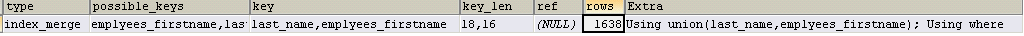
\includegraphics{5-1.png}

\begin{Verbatim}[commandchars=\\\{\}]
\PYG{k}{EXPLAIN} \PYG{k}{SELECT}
  \PYG{n}{emp\PYGZus{}no}\PYG{p}{,}
  \PYG{n}{first\PYGZus{}name}\PYG{p}{,}
  \PYG{n}{last\PYGZus{}name}\PYG{p}{,}
  \PYG{n}{hire\PYGZus{}date}
\PYG{k}{FROM}
  \PYG{n}{employees}
\PYG{k}{WHERE} \PYG{n}{last\PYGZus{}name} \PYG{o}{=} \PYG{l+s+s1}{\PYGZsq{}Demeyer\PYGZsq{}}
\PYG{k}{UNION}
\PYG{k}{SELECT}
  \PYG{n}{emp\PYGZus{}no}\PYG{p}{,}
  \PYG{n}{first\PYGZus{}name}\PYG{p}{,}
  \PYG{n}{last\PYGZus{}name}\PYG{p}{,}
  \PYG{n}{hire\PYGZus{}date}
\PYG{k}{FROM}
  \PYG{n}{employees}
\PYG{k}{WHERE} \PYG{n}{first\PYGZus{}name} \PYG{o}{=} \PYG{l+s+s1}{\PYGZsq{}Gao\PYGZsq{}}
\PYG{k}{LIMIT} \PYG{l+m+mi}{0}\PYG{p}{,} \PYG{l+m+mi}{1000000} \PYG{p}{;}
\end{Verbatim}

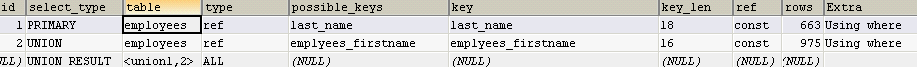
\includegraphics{5-2.png}


\chapter{性能优化}
\label{7/0::doc}\label{7/0:id1}

\section{编译器、文件格式、磁盘、索引结构}
\label{7/1::doc}\label{7/1:id1}
编译器改为ICC可以提升5\%,文件格式改为XFS可以提升5\%,增加1/6磁盘可以提升1/6,优化索引和结构一般可以提升100-1000


\section{使用type=heap的临时表}
\label{7/2:type-heap}\label{7/2::doc}
使用type=heap的临时表


\chapter{引擎使用}
\label{8/0::doc}\label{8/0:id1}

\section{innodb引擎,在过程结尾提交,避免过度commit}
\label{8/1::doc}\label{8/1:innodb-commit}
innodb引擎,在过程结尾提交,避免过度commit

\begin{Verbatim}[commandchars=\\\{\}]
\PYG{c+cp}{\PYGZlt{}?php}
\PYG{n+nv}{\PYGZdl{}conn} \PYG{o}{=} \PYG{n+nb}{mysql\PYGZus{}connect}\PYG{p}{(}\PYG{l+s+s1}{\PYGZsq{}localhost\PYGZsq{}}\PYG{p}{,}\PYG{l+s+s1}{\PYGZsq{}root\PYGZsq{}}\PYG{p}{,}\PYG{l+s+s1}{\PYGZsq{}root\PYGZsq{}}\PYG{p}{)} \PYG{k}{or} \PYG{k}{die} \PYG{p}{(}\PYG{l+s+s2}{\PYGZdq{}}\PYG{l+s+s2}{数据连接错误!!!}\PYG{l+s+s2}{\PYGZdq{}}\PYG{p}{);}
\PYG{n+nb}{mysql\PYGZus{}select\PYGZus{}db}\PYG{p}{(}\PYG{l+s+s1}{\PYGZsq{}test\PYGZsq{}}\PYG{p}{,}\PYG{n+nv}{\PYGZdl{}conn}\PYG{p}{);}
\PYG{n+nb}{mysql\PYGZus{}query}\PYG{p}{(}\PYG{l+s+s2}{\PYGZdq{}}\PYG{l+s+s2}{set names \PYGZsq{}GBK\PYGZsq{}}\PYG{l+s+s2}{\PYGZdq{}}\PYG{p}{);} \PYG{c+c1}{//使用GBK中文编码;}
\PYG{c+c1}{//开始一个事务}
\PYG{n+nb}{mysql\PYGZus{}query}\PYG{p}{(}\PYG{l+s+s2}{\PYGZdq{}}\PYG{l+s+s2}{BEGIN}\PYG{l+s+s2}{\PYGZdq{}}\PYG{p}{);} \PYG{c+c1}{//或者mysql\PYGZus{}query(\PYGZdq{}START TRANSACTION\PYGZdq{});}
\PYG{n+nv}{\PYGZdl{}sql} \PYG{o}{=} \PYG{l+s+s2}{\PYGZdq{}}\PYG{l+s+s2}{INSERT INTO {}`employees{}`.{}`employees{}` (}
\PYG{l+s+s2}{  {}`emp\PYGZus{}no{}`,}
\PYG{l+s+s2}{  {}`birth\PYGZus{}date{}`,}
\PYG{l+s+s2}{  {}`first\PYGZus{}name{}`,}
\PYG{l+s+s2}{  {}`last\PYGZus{}name{}`,}
\PYG{l+s+s2}{  {}`hire\PYGZus{}date{}`,}
\PYG{l+s+s2}{)}
\PYG{l+s+s2}{VALUES}
\PYG{l+s+s2}{  (}
\PYG{l+s+s2}{    99999,}
\PYG{l+s+s2}{    \PYGZsq{}1989\PYGZhy{}01\PYGZhy{}01,}
\PYG{l+s+s2}{    \PYGZsq{}first\PYGZus{}name\PYGZsq{},}
\PYG{l+s+s2}{    \PYGZsq{}last\PYGZus{}name\PYGZsq{},}
\PYG{l+s+s2}{     \PYGZsq{}1989\PYGZhy{}01\PYGZhy{}01\PYGZsq{}}
\PYG{l+s+s2}{  ) ;}\PYG{l+s+s2}{\PYGZdq{}}\PYG{p}{;}
\PYG{n+nv}{\PYGZdl{}sql2} \PYG{o}{=} \PYG{l+s+s2}{\PYGZdq{}}\PYG{l+s+s2}{delete from employees where emp\PYGZus{}no= \PYGZhy{}1}\PYG{l+s+s2}{\PYGZdq{}}\PYG{p}{;}\PYG{c+c1}{//这条我故意写错}
\PYG{n+nv}{\PYGZdl{}res} \PYG{o}{=} \PYG{n+nb}{mysql\PYGZus{}query}\PYG{p}{(}\PYG{n+nv}{\PYGZdl{}sql}\PYG{p}{);}
\PYG{n+nv}{\PYGZdl{}res1} \PYG{o}{=} \PYG{n+nb}{mysql\PYGZus{}query}\PYG{p}{(}\PYG{n+nv}{\PYGZdl{}sql2}\PYG{p}{);}
\PYG{k}{if}\PYG{p}{(}\PYG{n+nv}{\PYGZdl{}res} \PYG{o}{\PYGZam{}\PYGZam{}} \PYG{n+nv}{\PYGZdl{}res1}\PYG{p}{)\PYGZob{}}
\PYG{n+nb}{mysql\PYGZus{}query}\PYG{p}{(}\PYG{l+s+s2}{\PYGZdq{}}\PYG{l+s+s2}{COMMIT}\PYG{l+s+s2}{\PYGZdq{}}\PYG{p}{);}
\PYG{k}{echo} \PYG{l+s+s1}{\PYGZsq{}提交成功。\PYGZsq{}}\PYG{p}{;}
\PYG{p}{\PYGZcb{}}\PYG{k}{else}\PYG{p}{\PYGZob{}}
\PYG{n+nb}{mysql\PYGZus{}query}\PYG{p}{(}\PYG{l+s+s2}{\PYGZdq{}}\PYG{l+s+s2}{ROLLBACK}\PYG{l+s+s2}{\PYGZdq{}}\PYG{p}{);}
\PYG{k}{echo} \PYG{l+s+s1}{\PYGZsq{}数据回滚。\PYGZsq{}}\PYG{p}{;}
\PYG{p}{\PYGZcb{}}
\PYG{n+nb}{mysql\PYGZus{}query}\PYG{p}{(}\PYG{l+s+s2}{\PYGZdq{}}\PYG{l+s+s2}{END}\PYG{l+s+s2}{\PYGZdq{}}\PYG{p}{);}
\end{Verbatim}


\chapter{权限控制}
\label{9/0::doc}\label{9/0:id1}

\section{PHP连接MYSQL的用户只分配SIUD权限}
\label{9/1::doc}\label{9/1:phpmysqlsiud}
PHP连接MYSQL的用户只分配SIUD权限


\section{所有提交变量经过 mysql\_real\_escape\_string 进行转义}
\label{9/2::doc}\label{9/2:mysql-real-escape-string}
所有提交变量经过 mysql\_real\_escape\_string 进行转义,防止注入

\begin{Verbatim}[commandchars=\\\{\}]
\PYG{c+cp}{\PYGZlt{}?php}
\PYG{n+nv}{\PYGZdl{}con} \PYG{o}{=} \PYG{n+nb}{mysql\PYGZus{}connect}\PYG{p}{(}\PYG{l+s+s2}{\PYGZdq{}}\PYG{l+s+s2}{localhost}\PYG{l+s+s2}{\PYGZdq{}}\PYG{p}{,} \PYG{l+s+s2}{\PYGZdq{}}\PYG{l+s+s2}{hello}\PYG{l+s+s2}{\PYGZdq{}}\PYG{p}{,} \PYG{l+s+s2}{\PYGZdq{}}\PYG{l+s+s2}{321}\PYG{l+s+s2}{\PYGZdq{}}\PYG{p}{);}
\PYG{k}{if} \PYG{p}{(}\PYG{o}{!}\PYG{n+nv}{\PYGZdl{}con}\PYG{p}{)}
  \PYG{p}{\PYGZob{}}
  \PYG{k}{die}\PYG{p}{(}\PYG{l+s+s1}{\PYGZsq{}Could not connect: \PYGZsq{}} \PYG{o}{.} \PYG{n+nb}{mysql\PYGZus{}error}\PYG{p}{());}
  \PYG{p}{\PYGZcb{}}

\PYG{c+c1}{// 获得用户名和密码的代码}

\PYG{c+c1}{// 转义用户名和密码,以便在 SQL 中使用}
\PYG{n+nv}{\PYGZdl{}user} \PYG{o}{=} \PYG{n+nb}{mysql\PYGZus{}real\PYGZus{}escape\PYGZus{}string}\PYG{p}{(}\PYG{n+nv}{\PYGZdl{}user}\PYG{p}{);}
\PYG{n+nv}{\PYGZdl{}pwd} \PYG{o}{=} \PYG{n+nb}{mysql\PYGZus{}real\PYGZus{}escape\PYGZus{}string}\PYG{p}{(}\PYG{n+nv}{\PYGZdl{}pwd}\PYG{p}{);}

\PYG{n+nv}{\PYGZdl{}sql} \PYG{o}{=} \PYG{l+s+s2}{\PYGZdq{}}\PYG{l+s+s2}{SELECT * FROM users WHERE}
\PYG{l+s+s2}{user=\PYGZsq{}}\PYG{l+s+s2}{\PYGZdq{}} \PYG{o}{.} \PYG{n+nv}{\PYGZdl{}user} \PYG{o}{.} \PYG{l+s+s2}{\PYGZdq{}}\PYG{l+s+s2}{\PYGZsq{} AND password=\PYGZsq{}}\PYG{l+s+s2}{\PYGZdq{}} \PYG{o}{.} \PYG{n+nv}{\PYGZdl{}pwd} \PYG{o}{.} \PYG{l+s+s2}{\PYGZdq{}}\PYG{l+s+s2}{\PYGZsq{}}\PYG{l+s+s2}{\PYGZdq{}}

\PYG{c+c1}{// 更多代码}

\PYG{n+nb}{mysql\PYGZus{}close}\PYG{p}{(}\PYG{n+nv}{\PYGZdl{}con}\PYG{p}{);}
\end{Verbatim}



\renewcommand{\indexname}{Index}
\printindex
\end{document}
